\documentclass[10pt,conference]{IEEEtran}
\IEEEoverridecommandlockouts

% The preceding line is only needed to identify funding in the first footnote. If that is unneeded, please comment it out.
\usepackage[numbers,sort]{natbib}
\usepackage[colorlinks=true,citecolor=blue,linkcolor=blue,urlcolor=blue]{hyperref}
\usepackage{amsmath,amssymb,amsfonts}
\usepackage{algorithmic}
\usepackage{graphicx}
\usepackage{textcomp}
\usepackage{xcolor}
\usepackage{bm}
\usepackage{makecell}
\usepackage[linesnumbered,ruled,vlined]{algorithm2e}
\usepackage{caption}
\usepackage{color}
\usepackage{stfloats}
\usepackage{booktabs}
\usepackage{multirow}
\usepackage{verbatim}
\usepackage{bm}
\usepackage{url} %引用网页%
\usepackage{framed} % 文字加框
\usepackage{threeparttable}    %表格脚注左对齐
\usepackage{balance}  
\usepackage{color, colortbl}
\usepackage{enumitem}
	
\definecolor{Gray}{gray}{0.9}
\definecolor{LightCyan}{rgb}{0.88,1,1}

\captionsetup[table]{skip=5pt}

% save space
\usepackage{microtype}
\setlength\floatsep{0.2\baselineskip plus 3pt minus 2pt} % distance between two floats
\setlength\textfloatsep{0.2\baselineskip plus 3pt minus 2pt} % distance between floats on the top or the bottom and the text
\setlength\intextsep{0.2\baselineskip plus 3pt minus 2pt} % distance between floats inserted inside the text (using h) and the text
\setlength\dbltextfloatsep{0.2\baselineskip plus 3pt minus 2pt} % distance between a float spanning both columns and the text
\setlength\dblfloatsep{0.2\baselineskip plus 3pt minus 2pt} % distance between two floats spanning both columns.

\def\BibTeX{{\rm B\kern-.05em{\sc i\kern-.025em b}\kern-.08em
    T\kern-.1667em\lower.7ex\hbox{E}\kern-.125emX}}

\newcommand{\todo}[1]{\textcolor{black}{#1}}
\newcommand{\tabincell}[2]{\begin{tabular}{@{}#1@{}}#2\end{tabular}}

\begin{document}

\title{Characterizing the Complexity and Its Impact on Testing in ML-Enabled Systems \\ {\large A Case Sutdy on Rasa}}

%\author{\IEEEauthorblockN{Junming Cao}
%\IEEEauthorblockA{\textit{Fudan University} \\
%}
%\and
%\IEEEauthorblockN{Bihuan Chen}
%\IEEEauthorblockA{\textit{Fudan University} \\
%}
%\and
%\IEEEauthorblockN{Longjie Hu}
%\IEEEauthorblockA{\textit{Fudan University} \\
%}
%\and
%\IEEEauthorblockN{Jie Gao}
%\IEEEauthorblockA{\textit{Singapore University of Technology and Design} \\
%}
%\and
%\IEEEauthorblockN{Kaifeng Huang}
%\IEEEauthorblockA{\textit{Fudan University} \\
%}
%\and
%\IEEEauthorblockN{Xin Peng}
%\IEEEauthorblockA{\textit{Fudan University} \\
%}
%}
% \and
% \IEEEauthorblockN{4\textsuperscript{th} Xin Peng}
% \IEEEauthorblockA{\textit{dept. name of organization (of Aff.)} \\
% \textit{name of organization (of Aff.)}\\
% City, Country \\
% email address or ORCID}

\maketitle
%\IEEEpeerreviewmaketitle

\begin{abstract}
% !TeX root = ../main.tex
Machine learning (ML) enabled systems are emerging with recent breakthroughs in ML. A model-centric view is widely taken by the literature to focus only on the analysis~of~ML~models. However, only a small body of work takes a system view that~looks at how ML components work with the system and how they affect software engineering for ML-enabled systems. In this paper, we adopt this system view, and conduct~a~case study on Rasa~3.0,~an industrial dialogue system that has been widely adopted by various companies around~the world.~Our~goal~is~to~characterize~the~complexity of such a large-scale ML-enabled system~and~to~understand the~impact of the complexity on testing. Our study reveals~practical implications for software engineering for ML-enabled systems. 
\end{abstract}

%\begin{IEEEkeywords}
%machine learning system, empirical study
%\end{IEEEkeywords}

% !TeX root = ../main.tex

\section{introduction}
\vspace{-3pt}

The recent advances in machine learning (ML) have attracted an increasing interest in applying ML across a breadth~of~business domains, e.g., self-driving cars, virtual assistants, robotics, and health care. According to the Global AI Adoption~Index~by IBM~\cite{ibmreport}, 35\% of companies around the world have~deployed AI in their business, while 42\% of companies are exploring AI. Such a trend has caused the emergence of ML-enabled systems which are composed of ML and non-ML components.~ML~components are often important, but usually only a part of many components in ML-enabled systems~\cite{Christian2022}.

The previous research on software engineering~for machine learning often takes a model-centric view that~focuses~only~on the analysis of ML models~\cite{Christian2022, Katie2020}. For~example,~many~advances have been made for DL model testing~(e.g.,~\cite{Pei2017, Tian2018, Sun2018, Aggarwal2019, Kim2019, Feng2020, Zhang2020, Dola2021, ml_testing}),~verification~(e.g.,~\cite{Paulsen2020a, Toledo2021, Paulsen2020b, Baluta2021, Singh2019}) and debugging (e.g., \cite{Ma2018, Li2020, odena19a,Tao2020}). Only a small~body~of work takes a holistic system view, e.g., architectural design \cite{Yokoyama2019, Serban2022}, technical debt~\cite{hidden_technical_debt, tang2021empirical}, ML component entanglement \cite{Zhang2016, nushi2017human, fix_that_fails}, feature interaction \cite{Abdessalem2018, Abdessalem2020, feature_interaction}, and model interactions in Apollo~\cite{pengFirstLookIntegration2020}. However, the lack of system-level understanding of ML-enabled systems may hide problems in engineering ML-enabled systems and hinder practical solutions.

In this paper, we adopt this system view, and conduct~a~case study on Rasa 3.0 \cite{rasa} to characterize the complexity~of~such~a large-scale ML-enabled system as well as to understand~the~impact of the complexity on testing. Rasa is a task-oriented~industrial dialogue system that has been widely used by various companies around~the world. Therefore, we believe Rasa is a good representative of real-world ML-enabled systems. 

We first investigate~the~complexity of Rasa at three levels.~At the system level, we explore how ML components~are~adopted across the modules in Rasa. We find that there are~\todo{23}~ML~models in \todo{15} ML components across \todo{6} modules. At the interaction level,~we~analyze how ML components interact with other~components in Rasa. We find that there are \todo{43} interaction patterns and \todo{230} interaction instances across \todo{4} major categories and \todo{8} inner categories. At the component level, we investigate how the code of ML components is composed by what kinds~of~code. We find that \todo{57.1\%} of the code inside components are data processing code, and there are \todo{8} composition patterns between data processing code and model usage code.

We then explore the impact of the complexity on testing~from two perspectives. From the testing practice perspective,~we~analyze how is the characteristic of test cases, and how well~they cope with the complexity. We find that the test coverage~of~component interactions is low because of the complexity from huge configuration space and from hidden component interactions. From the mutation testing perspective, we study how~is~the~bug-finding capability of test cases and test data (i.e., the data for testing models), and how well they cope with the complexity. 
We find that there may be many potential bugs in data processing code that can only be detected by test cases, due to the complexity from data processing code.
The capability of test data to kill mutants is limited because of the complexity from huge configuration space.

Based on our case study, we highlight practical~implications to improve software engineering for ML-enabled~systems. For example, the configuration space of ML-enabled systems should be tested adequately, and configuration suggestions~should~be provided to developers.  A general taxonomy of data processing code should be constructed, and then the maintaining~and~testing tools for it can be developed. More integration-level test cases should be created to cover component interactions. Test cases and test data should be used in combination to detect both non-ML specific and ML-specific bugs.
% Test data is not 

In summary, this paper makes the following contributions.

\begin{itemize}
\item We conduct an in-depth case study on Rasa to characterize its complexity~and the~impact of its complexity on testing.
\item We highlight practical implications to improve software engineering for ML-enabled systems.
\end{itemize}

% !TeX root = ../main.tex

\section{Background and Study Design}
\vspace{-3pt}
We present the architecture of a typical task-oriented~dialogue systems, an overview of Rasa, and our study design.

\subsection{Architecture of a Typical Task-Oriented Dialogue System}

A task-oriented dialogue system (TDS) aims to assist~users~in performing specific tasks, such as restaurant booking~and~flight booking~\cite{multiwoz}. 
A pipeline-based TDS consists of four parts,~i.e., natural language understanding (NLU), dialogue state tracking (DST), dialogue policy (Policy) and natural language generation (NLG)~\cite{zhang2020recent}. 
NLU parses a user utterance~into~a~structured~semantic representation, including intent and slot-values.~The~intent is a high-level classification of the user utterance, such as \texttt{Inform} and \texttt{Request}. 
Slot-values are task-specific entities that are mentioned in the user utterance, such as restaurant~price range and location preference. 
After tokenization and featurization of the user utterance, NLU applies classification~models~to recognize intent, and named entity extraction models to extract slot-values. 
DST takes the entire history of the conversation, including both user utterances with predicted intents~and~slot-values and system responses, to estimate the current dialogue state, which is usually formulated as a sequential prediction~task \cite{williams2016dialogstate}.
Dialogue state is typically the probability distribution of user intent and slot-values till the current timestamp.~Given~the estimated dialogue state, Policy generates the next system~action, such as \texttt{Query Database} and \texttt{Utter Question}. 
As Policy determines a series of actions sequentially, sequential models such as Recurrent Neural Network (RNN) are applied. 
For actions that require a response, NLG converts the action into a natural language utterance, which is often considered as a sequence generation task~\cite{wen-etal-2015-semantically}.


\subsection{An Overview of Rasa 3.0}\label{sec:rasa_overview}

Rasa is a popular open-source ML-enabled TDS, which~is fully implemented with Python and used by many well-known companies in customer service for real users, including Adobe, Airbus, and N26 \cite{rasa}. 
An architecture overview~of~Rasa 3.0 is shown in Fig. \ref{overview_fig}. %A \textit{module} serves as a semantic function to transform given input into specific output, while 
Each module consists of one single component or multiple semantically similar components. 
%For example, there are multiple components inside \textit{Policy} module, which is implemented with ML models or rule-based code logic to predict the next system action. 
Apart from the modules in a typical TDS, Rasa proposes the Selector~module~to select candidate intents and responses for FAQ questions~\cite{chaudhuri-etal-2018-improving}.
We present some concepts in Rasa 3.0 to ease our presentation.

\textbf{Components in Rasa.} There are two types of components~in Rasa. We define \textit{ML components}~as~components that~are~implemented with ML models, and \textit{rule-based components} as components that are implemented with rule-based code logic.
General utils code in Rasa is not considered in this paper, such as command line and database access code.
% We consider rule-based components in this paper, because there may exist interactions between them and ML components. As a complex ML-enabled system, there exists inter-module and intra-module interactions among themselves, and a series of data processing code before and after the model usages within each component.

\textbf{Configuration File and Component Graph in Rasa.}~As there are multiple available components~in~each~module,~developers need to choose components that are actually used~in the Rasa pipeline with a \textit{configuration file} to build a chatbot. 
Parameters of each component~are~specified~in~the~configuration file (e.g., ML model used by a component~and hyperparamers of a ML model).
Rasa applies Dask~\cite{dask} to compile~a~configuration file into a component graph. 
Each node in the component~graph denotes a component, and the edges connected with it denote upstream and downstream components with input and output data dependency. 
Execution of components obeys~the~topological order specified by edges.
These components interact with each other through fields in shared \texttt{Message} class instances. %including \texttt{Message.sequence\_features}, \texttt{Message.intent} and \texttt{Message.entities}.
An upstream component stores outputs to \texttt{Message} instances, and a downstream component retrieves them for further processing. 

\textbf{ML Stages in Rasa.} 
Different from Apollo, which uses trained model files from external systems, and therefore~only contains the inference stage of ML models \cite{pengFirstLookIntegration2020}, the training, evaluation and inference stages of ML models are all~present in Rasa. 
Given a configuration file, Rasa separately compiles it to a training component graph and~an~inference~component graph. 
% which specify the methods in components that should be invoked in these stages.
In training stage, the trainable~upstream~components are first trained, and then process the training data used by downstream components. 
%For example, the \textit{CountVectorsFeaturizer} component is trained first, and then the \texttt{process\_training\_data} of it is called to create features for classifiers to be traind.
In evaluation stage, only the performance metrics of \textit{IntentClassifier}, \textit{EntityExtractor} and \textit{Policy} are reported, as there is no ground truth for evaluation data in other modules.


%\textbf{Test Cases in Rasa.} 
%Rasa provides a test suite of~47~test files and 461 test functions for ML-related code. We consider each test function as a test case. These test cases target at different granularity levels, including method-level, component-level and integration-level.
%There are four types of test oracles, including given input-output pairs, component-specific constraints, differential executions and exception oracles. 
%All three previously mentioned ML stages are tested.
%To test the training stage of a component, test cases must first train it  and check whether any test oracle is violated.
%The statistics of test cases are presented in Section \ref{sec:test_case}.


\subsection{Study Design}

Our goal is to understand the complexity and its impact on testing in Rasa. To achieve this goal, we propose five RQs. %the first three research questions to characterize the complexity at three levels and the last two research questions to investigate its impact on testing as follows.

\begin{itemize}[leftmargin=*]
    \item \textbf{RQ1 System Complexity Analysis}: how ML components~are adopted across the modules in Rasa?
    \item \textbf{RQ2 Interaction Complexity Analysis}: how ML components interact with other~components in Rasa?
    \item \textbf{RQ3 Component Complexity Analysis}: how the code of ML components is composed by what kinds~of~code?
    \item \textbf{RQ4 Testing Practice Analysis}: how is the characteristic of test cases, and how well~they cope with the complexity?
    \item \textbf{RQ5 Mutation Testing Analysis}: how~is~the~bug-finding capability of test cases and test data (i.e., the data for testing models), and how well they cope with the complexity?
\end{itemize}

\textbf{RQ1} aims to identify ML components in Rasa and broadly view them from the perspective of dependent libraries and ML models. 
\textbf{RQ2} aims to summarize a comprehensive taxonomy of component interaction patterns. 
\textbf{RQ3} aims to inspect the source code inside every component to characterize the statistics and composition patterns of different code types, including data processing code, model usage code, etc. 
Our findings from \textbf{RQ1}, \textbf{RQ2} and \textbf{RQ3} could reveal how the complexity originates and manifests in real world large-scale ML-enabled systems, which provide both practitioners and researchers with insights to overcome the complexities involved in implementing, maintaining, debugging and testing such complex systems. 

\textbf{RQ4} aims to quantitatively assess Rasa's test cases from~code coverage, test case statistics (i.e., granularity levels, oracle~types, and ML stages), and component interaction coverage perspectives. 
\textbf{RQ5} aims to generate mutants (i.e., artificial bugs) and check whether these mutants can be killed (i.e., detected) by test cases. 
Further, for the survived mutants, we train~Rasa~with 3 default configuration files on \textit{MutiWoz} \cite{multiwoz}, a widely used multi-domain TDS dataset. 
We calculate the statistical significance between the performance metrics from mutated Rasa code with metrics from pipelines trained with clean code.
Our findings from \textbf{RQ4} and \textbf{RQ5} evaluate the testing practice in Rasa, and shed light on automated test generation, bug localization and bug repairing techniques for complex ML-enabled systems.


\begin{figure*}[!t]
\centering
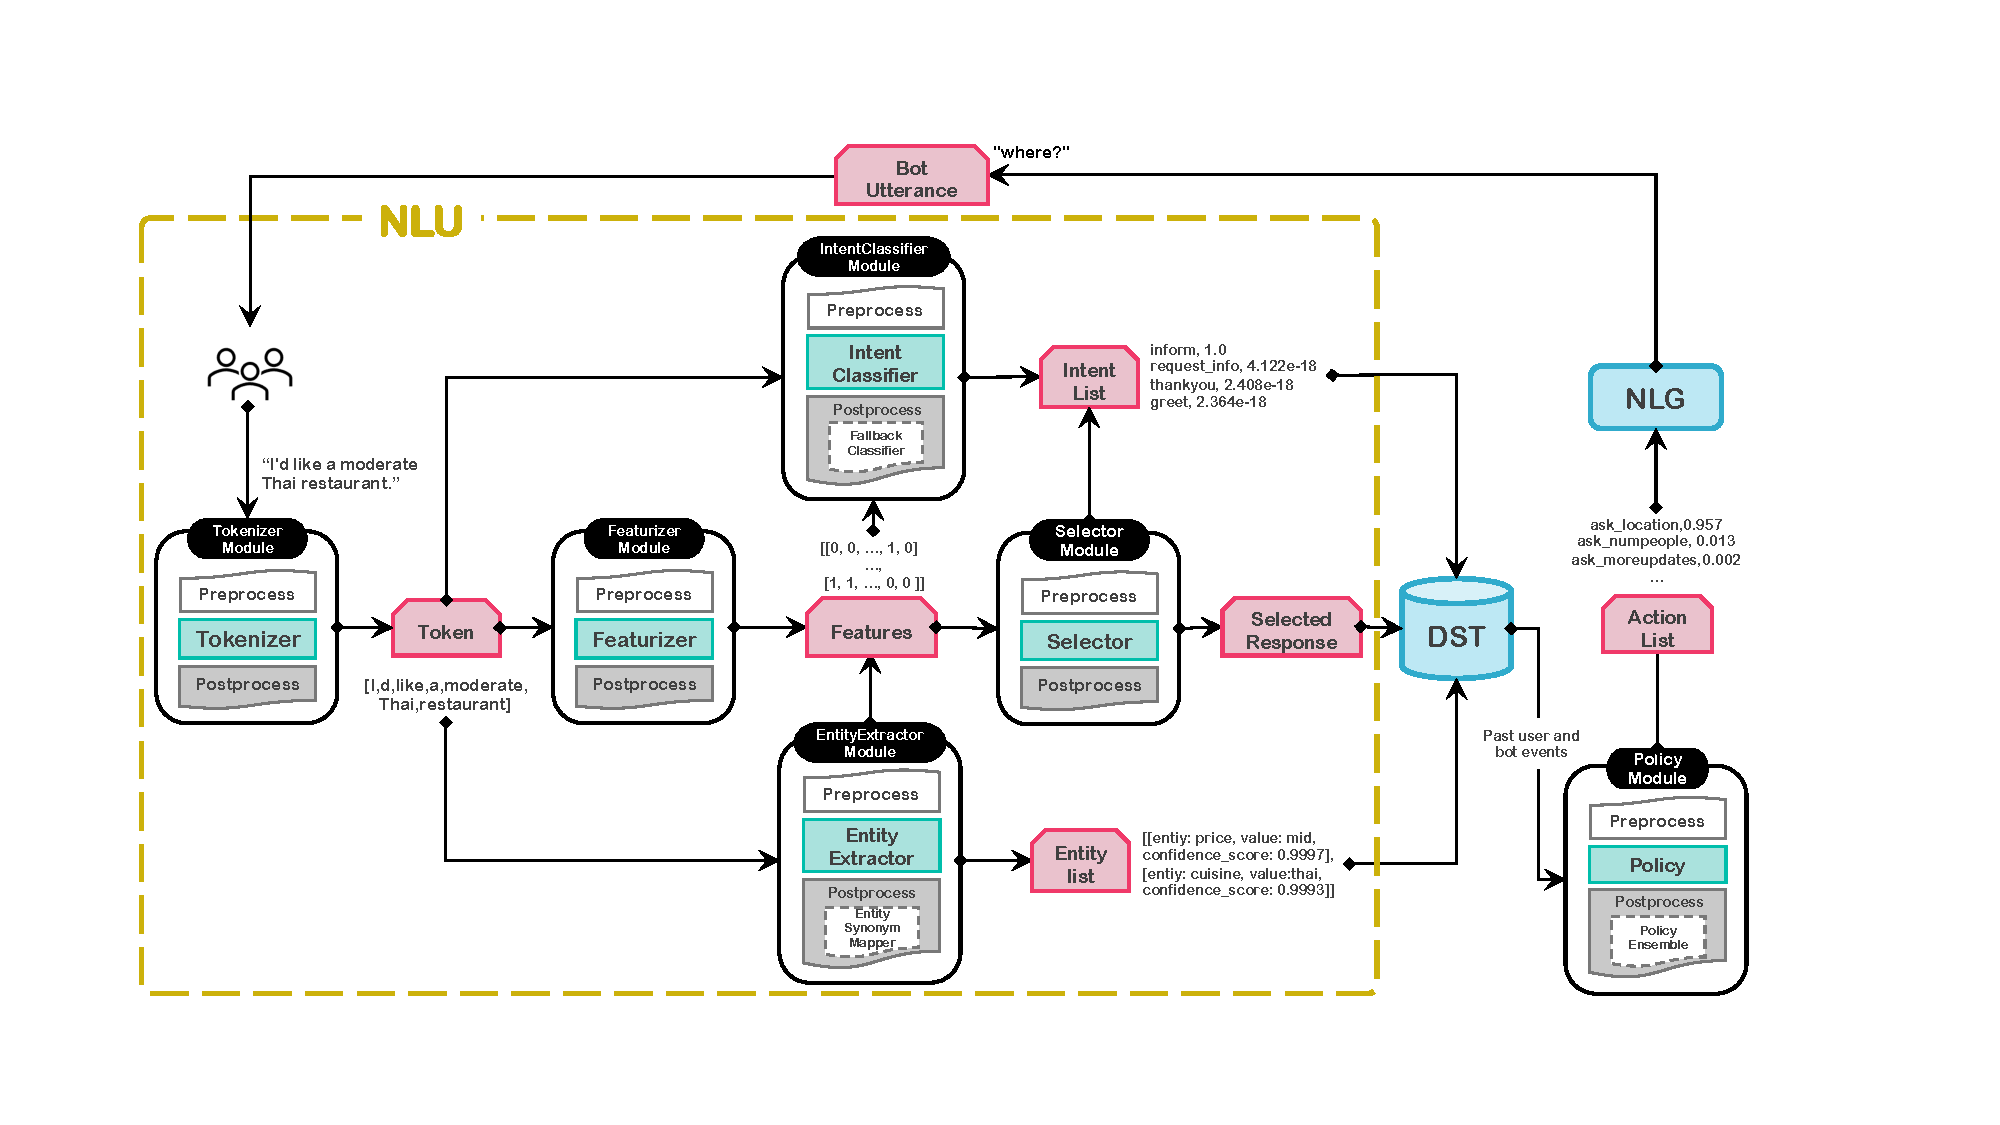
\includegraphics[scale=0.60]{figs/overview.pdf}
\caption{The Modules and Workflow of Rasa}\label{overview_fig}
\end{figure*}

\begin{table*}[!h]
	\caption{System Complexity Analysis of Rasa}
	\vspace{-10pt}
	\begin{center}
        \scalebox{0.97}{
	\begin{tabular}{llllllllll}
	\toprule
	\textbf{Module}
	& \textbf{Component}
	& \textbf{Direct Lib.}
	& \textbf{Indirect Lib.}
	& \textbf{Model Type}
	& \textbf{No. Model}
    & \textbf{Trainable}
    & \textbf{Rasa Imp.}
    & \textbf{LoC}\\
	\midrule
	\multirow{4}*{Tokenizer}
	&\cellcolor{Gray}JiebaTokenizer & \cellcolor{Gray}Jieba &\cellcolor{Gray}N/A &\cellcolor{Gray}HMM & \cellcolor{Gray}1 &\cellcolor{Gray}False  &\cellcolor{Gray}False   &\cellcolor{Gray}85  \\
	&\cellcolor{Gray}SpacyTokenizer &\cellcolor{Gray}Spacy &\cellcolor{Gray}Thinc &\cellcolor{Gray}MLP &\cellcolor{Gray}1 &\cellcolor{Gray}False  &\cellcolor{Gray}False &\cellcolor{Gray}39  \\
	&MitieTokenizer &Mitie &N/A &N/A &N/A &False  &False &43  \\
    &WhitespaceTokenizer &N/A &N/A &N/A &N/A &False &True &52    \\
	\midrule
	\multirow{7}*{Featurizer}
	&\cellcolor{Gray}ConveRTFeaturizer &\cellcolor{Gray}TensorFlow &\cellcolor{Gray}N/A &\cellcolor{Gray}Transformer &\cellcolor{Gray}1 &\cellcolor{Gray}False &\cellcolor{Gray}False &\cellcolor{Gray}269 \\
	&\cellcolor{Gray}LanguageModelFeaturizer &\cellcolor{Gray}Transformers &\cellcolor{Gray}TensorFlow &\cellcolor{Gray}Transformer &\cellcolor{Gray}6 &\cellcolor{Gray}False &\cellcolor{Gray}False &\cellcolor{Gray}378  \\
	&\cellcolor{Gray}MitieFeaturizer &\cellcolor{Gray}Mitie &\cellcolor{Gray}Dlib &\cellcolor{Gray}CCA &\cellcolor{Gray}1 &\cellcolor{Gray}False &\cellcolor{Gray}False &\cellcolor{Gray}98   \\
    &\cellcolor{Gray}SpacyFeaturizer &\cellcolor{Gray}Spacy &\cellcolor{Gray}Thinc &\cellcolor{Gray}CNN &\cellcolor{Gray}2 &\cellcolor{Gray}False &\cellcolor{Gray}False &\cellcolor{Gray}66   \\
    &CountVectorsFeaturizer &Scikit-learn &N/A &N/A &N/A &True &False &520   \\
    &LexicalSyntacticFeaturizer &N/A &N/A &N/A &N/A &True  &True &319  \\
    &RegexFeaturizer &N/A &N/A &N/A &N/A &True &True &151  \\
    \midrule
    \multirow{5}*{IntentClassifier}
    &\cellcolor{Gray}DIETClassifier &\cellcolor{Gray}TensorFlow &\cellcolor{Gray}N/A &\cellcolor{Gray}Transformer &\cellcolor{Gray}1 &\cellcolor{Gray}True &\cellcolor{Gray}True &\cellcolor{Gray}1217 \\
    &\cellcolor{Gray}MitieIntentClassifier &\cellcolor{Gray}Mitie &\cellcolor{Gray}Dlib &\cellcolor{Gray}SVM &\cellcolor{Gray}1 &\cellcolor{Gray}True &\cellcolor{Gray}False &\cellcolor{Gray}89 \\
    &\cellcolor{Gray}SklearnIntentClassifier &\cellcolor{Gray}Scikit-learn &\cellcolor{Gray}N/A &\cellcolor{Gray}SVM &\cellcolor{Gray}1 &\cellcolor{Gray}True &\cellcolor{Gray}False &\cellcolor{Gray}173 \\
    &FallbackClassifier  &N/A &N/A &N/A &N/A &False &True&91   \\
    &KeywordIntentClassifier  &N/A &N/A &N/A &N/A &True &True&132  \\
    \midrule
    \multirow{7}*{EntityExtractor}
    &\cellcolor{Gray}DIETClassifier &\cellcolor{Gray}TensorFlow &\cellcolor{Gray}N/A &\cellcolor{Gray}Transformer &\cellcolor{Gray}1 &\cellcolor{Gray}True &\cellcolor{Gray}True &\cellcolor{Gray}1217 \\
    &\cellcolor{Gray}CRFEntityExtractor &\cellcolor{Gray}Scikit-learn &\cellcolor{Gray}N/A &\cellcolor{Gray}CRF &\cellcolor{Gray}1 &\cellcolor{Gray}True &\cellcolor{Gray}False &\cellcolor{Gray}438 \\
    &\cellcolor{Gray}MitieEntityExtractor &\cellcolor{Gray}Mitie &\cellcolor{Gray}Dlib &\cellcolor{Gray}SVM &\cellcolor{Gray}1 &\cellcolor{Gray}True &\cellcolor{Gray}False &\cellcolor{Gray}164 \\
    &\cellcolor{Gray}SpacyEntityExtractor  &\cellcolor{Gray}Spacy &\cellcolor{Gray}Thinc &\cellcolor{Gray}MLP &\cellcolor{Gray}1 &\cellcolor{Gray}False  &\cellcolor{Gray}False &\cellcolor{Gray}52  \\
    &DucklingEntityExtractor  &N/A &N/A &N/A &N/A &False &False &134   \\
    &RegexEntityExtractor &N/A &N/A &N/A &N/A &True  &True &124  \\
    &EntitySynonymMapper &N/A &N/A &N/A &N/A &True  &True &102  \\
    \midrule
    Selector
    &\cellcolor{Gray}ResponseSelector &\cellcolor{Gray}TensorFlow &\cellcolor{Gray}N/A &\cellcolor{Gray}Transformer &\cellcolor{Gray}2 &\cellcolor{Gray}True &\cellcolor{Gray}True &\cellcolor{Gray}560  \\
    \midrule
    \multirow{6}*{Policy}
    &\cellcolor{Gray}TEDPolicy &\cellcolor{Gray}TensorFlow &\cellcolor{Gray}N/A &\cellcolor{Gray}Transformer+CRF &\cellcolor{Gray}1 &\cellcolor{Gray}True &\cellcolor{Gray}True &\cellcolor{Gray}1262 \\
    &\cellcolor{Gray}UnexpecTEDIntentPolicy &\cellcolor{Gray}TensorFlow &\cellcolor{Gray}N/A &\cellcolor{Gray}Transformer+CRF &\cellcolor{Gray}1 &\cellcolor{Gray}True &\cellcolor{Gray}True &\cellcolor{Gray}458 \\
    &MemoizationPolicy &N/A &N/A &N/A &N/A &True &True &207   \\
    &AugmentedMemoizationPolicy &N/A &N/A &N/A &N/A &True &True &65   \\
    &RulePolicy &N/A &N/A &N/A &N/A &True &True &818   \\
    &PolicyEnsemble &N/A &N/A &N/A &N/A &False &True &150   \\
	\bottomrule
	\end{tabular}		
	\label{system_complexity}}
	\end{center}
\end{table*}

% !TeX root = ../main.tex

\section{RQ1: System Complexity Analysis}
\vspace{-3pt}

\subsection{Methodology}

To answer \textbf{RQ1}, we identified and characterized ML and rule-based components in Rasa through an in-depth analysis of its source code and documentation. We excluded DST and NLG as they are fully implemented with rule-based code logic in Rasa without ML components. 

All the modules we identified are listed in Table \ref{system_complexity}, except for a special module, \textit{Shared}, as it contains general data processing code and  ML model definition code (e.g., Transformer), while does not contain any independent components. We will consider it in the last three RQs. Specifically, for each component, we recursively tracked methods within it to manually extract the model or rule definition code. We investigated the implementation details of APIs in ML libraries by examining the documentation and source code of external libraries, including ML model type and number of candidate models. 

In particular, we analyzed if ML components are implemented using direct or indirect external libraries, whether the components can be trained (notice that not only some of ML components can be trained, but also certain rule-based components, as long as they update internal parameters when processing training data),  whether Rasa implements components with its own code and provides built-in model and rule definition code, and the lines of code (LoC) of each component, excluding blank lines, code comments and import statements. 

%\textit{Direct Lib.}: External ML libraries used to implement ML components;

%\textit{Indirect Lib}.: Lower-level ML libraries relied by above mentioned external ML libraries;

% \textit{Trainable}: Whether the component can be trained. In particular, not only some of ML components can be trained, but also some rule-based components as long as they update internal parameters when processing training data; 

% \textit{Rasa Imp.}: Whether Rasa implements components with its own code and provides built-in model and rule definition code; 

% \textit{LoC}: Lines of code (LoC) of each component excluding blank lines, code comments and import statements. 


\subsection{Results}

The results are summarized in Table \ref{system_complexity}.
Components shown in gray color are ML components, while others are rule-based components. In total,
there are 6 modules, consisting of 15 ML and 14 rule-based components. These components encompass 23 ML models and are implemented with 7 directly dependent external ML libraries and 3 indirectly dependent external ML libraries. Notably, all ML components in \textit{Tokenizer} and \textit{Featurizer} are non-trainable as they utilize pre-trained language models. All components in \textit{Policy} are implemented in Rasa's own code, because no ready-to-use Policy models are provided by existing libraries. There are a total of 5348 LoC in ML components and 2980 LoC in rule-based components. In addition, the general module \textit{Shared} contains 5375 LoC, which is not listed in the table.

Notably, we discovered that classical machine learning models (e.g., Support Vector Machine and Conditional Random Field) and deep learning models (e.g., Convolutional Neural Networks and Transformer) both play an important role in Rasa. This contrasts with the previous study \cite{pengFirstLookIntegration2020} on Apollo, which primarily focused on deep learning models.


Next, we introduce the components used in each module.

\textbf{Tokenizer.} Tokenizer splits the user utterance into tokens with component specific split symbols (e.g., whitespace and punctuation). (1) \textit{SpacyTokenizer} provides the richest token information, including splitting tokens with rules, lemmatizing tokens with a look-up table, and performing part-of-speech~tagging with a multi-layer perceptron (MLP). 
(2) \textit{JiebaTokenizer} is the only component that tokenizes non-English sentences using Hidden Markov Model (HMM) \cite{eddy1996hidden}. (3) \textit{MitieTokenizer} and \textit{WhitespaceTokenizer} toeknize text with predefined rules.
% The lemmatization and Part-of-Speech tags can be used by \textit{CountVectorsFeaturizer} and \textit{LexicalSyntacticFeaturizer} respectively.
% \textit{MitieTokenizer} tokenizes the text in the same way as the CoNLL 2003 dataset was tokenized with rules. \todo{Add reference of CoNLL 2003 dataset.} \textit{WhitespaceTokenizer} is the only tokenizer that implemented in Rasa source code. It tokenizes sentences and removes emoji tokens with regex patterns.

\textbf{Featurizer.} As shown in Fig. \ref{overview_fig}, Featurizer converts tokens into features for downstream module inference. (1) \textit{ConveRTFeaturizer} loads TFHub's \cite{TensorHub} pre-trained ConveRT (Conversational Representations from Transformers) TensorFlow model  to featurize tokens \cite{henderson2019convert}. (2) \textit{LanguageModelFeaturizer} loads pre-trained language models from Hugging Face Transformers \cite{transformers}, including BERT \cite{devlin2018bert}, GPT \cite{hu2020gpt}, XLNet \cite{yang2019xlnet}, Roberta \cite{liu2019roberta}, XLM \cite{xlm} and GPT2 \cite{gpt2}.
(3) \textit{MitieFeaturizer} combines Canonical Correlation Analysis (CCA) feature and word~morphology features together. (4) \textit{SpacyFeaturizer} applies HashEmbedCNN or Roberta to convert tokens to features, depending on the pre-trained Spacy pipeline specified in the configuration file.
(5) \textit{CountVectorsFeaturizer}, \textit{LexicalSyntacticFeaturizer} and \textit{RegexFeaturizer} create sparse features with n-grams, sliding window and regex patterns,  respectively. 
% It can be divided into \textit{DenseFeaturizer} and \textit{SparseFeaturizer}, which generate features first and then store them with dense matrix and sparse matrix, respectively. Also, components of \textit{DenseFeaturizer} are implemented with unsupervised pre-trained word embedding models(e.g. BERT), and contain all ML components in \textit{Featurizer}. \todo{Add reference of word2vec.} 
% Components of \textit{SparseFeaturizer} are implemented with rules to create features of tokens.


% \textit{CountVectorsFeaturizer} creates bad-of-words representation of tokens with Scikit-learn, and can be configured to use word or character n-grams.
% \textit{LexicalSyntacticFeaturizer} creates lexical and syntactic features for \textbf{EntityExtractor}, moving over the tokens with a sliding window to extract features like if the token is at the beginnning of the sentence and if the token is lower case. 
% With regex patterns defined in training data, \textit{RegexFeaturizer} creates features to denote whether these patterns exist in current tokens. 

\textbf{IntentClassifier.} IntentClassifier generates a predicted intent list ordered by confidence scores based on tokens and features from upstream modules.
(1) \textit{DIETClassifier} implements Dual Intent and Entity Transformer (DIET) to perform intent~classification and entity recognition simultaneously, and is therefore included in both \textbf{IntentClassifier} and \textbf{EntityExtractor} modules. % With this in mind, the following analysis considered \textit{DIETClassifier} in both modules but only counted once in the overall summarized results.
(2) \textit{MitieIntentClassifier} and \textit{SklearnIntentClassifier} apply a multi-class Support Vector Machine (SVM) \cite{Shmilovici2005} with a sparse linear kernel using Scikit-learn and Mitie, respectively.
(3) \textit{KeywordIntentClassifier} classifies  user intent with keywords extracted from training data.
% \textit{MitieIntentClassifier} applies a multi-class linear Support Vector Machine (SVM) with a sparse linear kernel to perform intent classification.
% \textit{SklearnIntentClassifier} trains a linear SVM with grid search to find the best hyperparameters set.
% \textit{KeywordIntentClassifier} takes training examples for an intent as keywords of it. This means the entire example is the keyword, not the individual words in the example is used to be matched against the user utterance. This component is not scalable and robust, thus is only intented in small projects or to get started.
(4) \textit{FallbackClassifier} is a post-processing component to check the results of other components in \textit{DIETClassifier}. It identifies a user utterance with the intent \texttt{nlu\_fallback} if the confidence scores are not greater than  \texttt{threshold}, or the score difference of the two highest ranked intents is less than the \texttt{ambiguity\_threshold}.

\textbf{EntityExtractor.} EntityExtractor extract entities such as the restaurant's location and price. (1) \textit{DIETClassifier} also serves as an EntityExtractor. 
% \textit{CRFEntityExtractor} utilizes a conditional random fields (CRF) model from Scikit-learn to perform named entity recognition. \textit{MitieEntityExtractor} applies a multi-class linear SVM with a sparse linear kernel to extract entities, but does not provide entity confidence values. \textit{SpacyEntityExtractor} is the only non-trainable ML-based EntityExtractor, which uses a MLP to predict the entities. 
(2) \textit{CRFEntityExtractor}, \textit{MitieEntityExtractor} and \textit{SpacyEntityExtractor} utilize a conditional random fields (CRF) model, a multi-class linear SVM, and a MLP to predict entities, respectively. 
(3) \textit{DucklingEntityExtractor} and \textit{RegexEntityExtractor} extract entities using a duckling server \cite{duckling} and regex patterns.
% \textit
% {DucklingEntityExtractor} extracts common entities like dates and amounts of money with a duckling server \cite{duckling}. \textit{RegexEntityExtractor} extracts entities using the lookup tables and regex patterns defined in the training data. 
(4) \textit{EntitySynonymMapper} is a post-processing component to convert synonymous entity values~into a same value. As Fig. \ref{overview_fig} shows, the value of ``price" entity, ``moderate", is coverted to ``mid" by \textit{EntitySynonymMapper}.

\textbf{Selector.} \textit{ResponseSelector} aims to directly select the response from a set of candidate responses, which is also known as response selection task in the literature \cite{chaudhuri-etal-2018-improving}. It embeds user inputs and candidate responses in the same vector space, using the same neural network architecture as \textit{DIETClassifier}.

\textbf{Policy.} Policy decides the action the system takes on each conversation based on dialogue states.
(1) \textit{TEDPolicy} proposes a Transformer Embedding Dialogue (TED) model to embed dialogue states and system actions into a single~semantic~vector space, and select the action with the max similarity score~with the current dialogue states \cite{TED}.
(2) \textit{MemoizationPolicy}, \textit{AugmentedMemoizationPolicy} and \textit{RulePolicy} match the current conversation history with examples in the training data and predefined rules to predict system actions.
% \textit{MemoizationPolicy} checks if the current conversation history matches any example in the training data, and predicts the next action accroding to the matched training example. \textit{AugmentedMemoizationPolicy} is extended from \textit{MemoizationPolicy}, because it has a forgetting mechanism that will forget a certain amount of steps of the curent conversation and match the reduced history with training example.
% \textit{RulePolicy} matchs conversations with pre-defined rules, which specify lists of user intents, entities, and corresponding system actions in order. 
(3) \textit{UnexpecTEDIntentPolicy} decides on the possibility of the intent predicted by IntentClassifier given current dialogue states, which follows the same model architecture as \textit{TEDPolicy}.
(4) \textit{PolicyEnsemble} is a post-processing component to select the proper system action from output actions of different policies. 
% It selects the system action with the highest confidence score, and selects according to the priority of policies if there are multiple policies that predict actions with the highest confidence score. 
% The components order from high priority to low is \textit{RulePolicy}, \textit{MemoizationPolicy}, \textit{AugmentedMemoizationPolicy}, \textit{UnexpecTEDIntentPolicy} and \textit{TEDPolicy}  


\subsection{Implications}

The system complexity of Rasa presents challenges for both developers utilizing Rasa (i.e., application developers) and those creating Rasa (i.e., system developers).

\textbf{Complexity from ML supply chain.} Rasa depends~on~10 external ML libraries either directly or indirectly. Fewer than~100~(0.03\%) projects out of 355392 projects using TensorFlow on GitHub depend on 10 more DL libraries \cite{supply_chain}. This suggests that relying on 10 or more ML libraries is relatively uncommon.
For application developers, understanding the implementation details of components that rely on external ML libraries is challenging, not to mention selecting proper components and parameters. For example, due to insufficient documentation for \textit{MitieFeaturizer} in Rasa, application developers must inspect Mitie's source code to learn that it implements CCA using Dlib APIs. 
% and combines the CCA feature with word morphology features.
For system developers, vulnerabilities \cite{npm_technical_lag} and dependency bugs \cite{dependency_bug} may emerge as a result of outdated or incompatible library versions. 
Therefore, future work should provide supports for managing components and their corresponding dependent ML libraries in ML-enabled systems, similar to traditional software component analysis \cite{Foo2019TheDO}.

\textbf{Complexity from configurations.} Configuring Rasa with 29 components and hundreds of parameters can be incredibly complex, leading to potential misconfigurations that may impact functionality and performance. This type of misconfiguration is similar to what occurs in traditional configurable software systems \cite{configurable_system}. Furthermore, finding optimal configurations for specific TDS scenarios is challenging for application developers,~also known as configuration debt \cite{hidden_technical_debt}. Although AutoML~has~been extensively studied to select appropriate ML models~and~parameters for specific tasks, they all focus on selecting a single ML model without considering the combination of multiple ML models and rules  \cite{XinHe2021AutoMLAS}. Another challenge~is~to~detect~potential bugs by testing a huge set of configuration settings. Existing studies on ML model testing primarily focus on testing a single ML model with predefined hyperparameters \cite{ml_testing}.
 
% \textbf{Complexity from long ML pipeline.} 
% \textbf{Complexity from different ML stages.} Different from Apollo.
% Trainable. indroduce additional complexity.
% !TeX root = ../main.tex

\section{RQ2: Interaction Complexity Analysis}
\vspace{-3pt}
\subsection{Methodology}

The workflow in Fig.~\ref{overview_fig} only shows the general~flow~among different modules. The details of interactions among components are still uncovered. We consider the interaction among two or more components, with at least one ML component.
An interaction pattern contains a module placeholder, which could be instantiated with components in the module~to~generate~interaction instances.
For example, pattern (PolicyEnsemble, [Policy]) could be instantiated as (PolicyEnsemble, TEDPolicy) or (PolicyEnsemble, (TEDPolicy, RulePolicy)). To answer \textbf{RQ2}, we conducted a qualitative and quantitative analysis of the component interaction patterns and instances of components.

\textbf{Step 1: Extract interaction patterns.}
The interaction can be divided into two categories: inter-module interaction and intra-module interaction.
(1) Inter-module interaction: the interaction between two adjacent modules (e.g., Featurizer with Tokenizer) was considered. We analyzed the usages~of~\texttt{Message} in the component code, as components use the \texttt{Message} class to transfer data. Specifically, we extracted all interaction patterns of its upstream and downstream components. We also considered the interaction between post-processing components (i.e., \textit{FallbackClassifier}, \textit{EntitySynonymMapper} and \textit{PolicyEnsemble}) and other components in their residing modules as inter-module interaction.
(2) Intra-module interaction: we identified interaction patterns for components within each module.

\textbf{Step 2: Generate interaction instances.}
For each inter-module interaction pattern, we instantiated the module placeholder with every component in the module. 
For every intra-module interaction, we derived the Cartesian product~of~all components in each module as interaction instances.
We~then filtered out component instances that do not contain ML~components, or do not meet the constraints specified~in~Rasa~documentation. 
For example, \textit{CRFEntityExtractor} could not use features of \textit{SparseFeaturizer} other than \textit{RegexFeaturizer}.
% For example, \textit{PolicyEnsemble} could interagete one, two or more Policies.

\textbf{Step 3: Summarize the interaction taxonomy.} For generated component patterns and instances, we analyzed their semantics and summarized a component interaction taxonomy.

\subsection{Results}
\begin{figure}[!t]
    \centering
    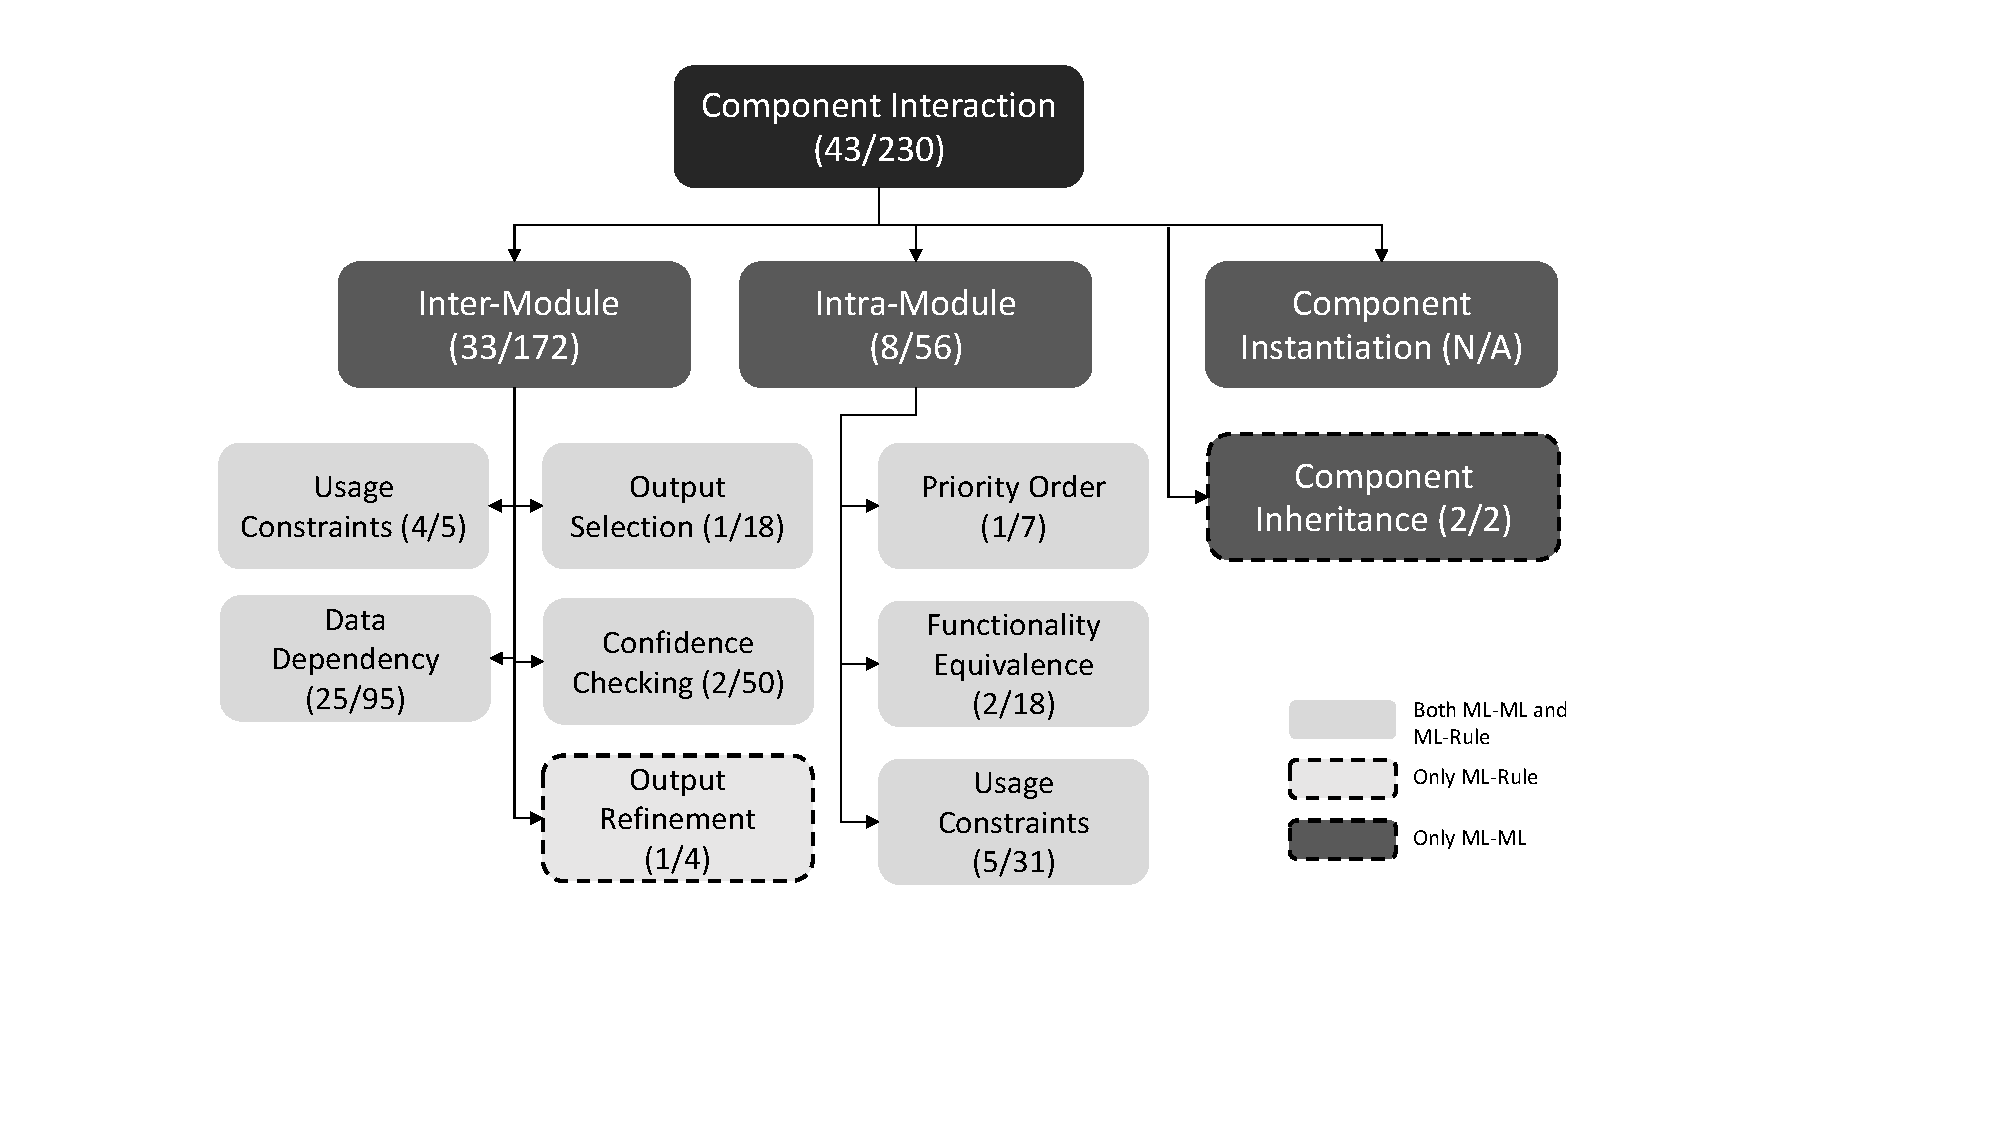
\includegraphics[scale=0.38]{figs/component_interaction.pdf}
    \caption{Taxonomy of Component Interactions}
    \label{component_interaction_fig}
\end{figure}

The component interaction taxonomy is shown in Fig. \ref{component_interaction_fig}. It is divided into 4 high-level categories (i.e. \textit{Inter-Module}, \textit{Intra-Module}, \textit{Component Instantiation} and \textit{Component Inheritance}) and 8 inner categories. 
Note that only \textit{Inter-Module} interactions contain components with direct data dependencies, while other categories contain components with indirect interactions (e.g., two featurizers are used together). The number of interaction patterns and interaction instances in each category~is~listed~as \textit{pattern\_count}/\textit{instance\_count} in Fig. \ref{component_interaction_fig}. There are a total of 43 interaction patterns and 230 interaction instances.
Nearly all categories include both ML to ML components and ML to rule-based components interactions. On the contrary, previous work on Apollo \cite{pengFirstLookIntegration2020} also presented 4 of the 8 inner categories, but did not provide a taxonomy and quantitative analysis. 

% \todo{Question: whther add number propertion of each category?}
% \todo{2 types of interaction covered in Apollo analysis.}

\textbf{Inter-Module}. Components from multiple modules interact through data transfers. In particular, \textit{Output Selection} means that the downstream component selects the proper output from multiple upstream outputs based on configurable criteria, e.g., \textit{PolicyEnsemble} with policies. 
\textit{Output Refinement} denotes that the downstream component complements the imperfect outputs of upstream components with rules, e.g., 
\textit{EntitySynonymMapper} with entity extractors. \textit{Confidence Checking} means that the downstream component checks reliability of the output from upstream components using ML models (e.g., \textit{UnexpecTEDIntentPolicy} with intent classifiers) or rules (e.g., \textit{FallbackClassifier} with IntentClassifiers). If the outputs are marked as not reliable, fallback behaviors such as the \texttt{fall\_back} system action are triggered. 
% \todo{Question: these compoenets are in the same module in Table I. and the functionability of them have been described in RQ1}.
\textit{Usage Constraints} defines components that should or should not be used together under certain circumstances. For example, \textit{SpacyTokenizer} is required by \textit{CountVectorsFeaturizer} when applying \texttt{use\_lemma} option and \textit{LexicalSyntacticFeaturizer} when applying \texttt{pos\_tag} option. \textit{Data Dependency} includes the rest of inter-module interaction patterns that do not fall into any of the above categories, which are relatively ``trivial" interactions with no specific semantics.

\textbf{Intra-Module}. The interaction mode of components within a module differs from \textbf{Inter-Module}. These components interact indirectly when used together. 
\textit{Priority Order} means that the outputs of components within a module are selected according to priority order, e.g., the priority order of policies.
\textit{Usage Constraints} is similar to \textit{Usage Constraints} in the inter-module category. For example, only one component in any of \textit{Tokenizer}, \textit{IntentClassifier} and \textit{EntityExtractor} should be used in each configuration file, otherwise outputs of additional components will be overwritten.  \textit{Functionality Equivalence} includes all intra-module interaction patterns that do not belong to any of the above categories, which are relatively ``trivial" interactions involving components used together with no specific semantics.

\textbf{Component Instantiation}. Rasa supports creating multiple instances of a component within a configuration setting. For example, multiple \textit{CountVectorFeaturizers} instances with different ngram settings, and multiple \textit{LanguageModelFeaturizer} instances with different language models could be used together. We did not count this category of interaction patterns and instances, since developers could specify infinite instances of a component within a configuration setting.

\textbf{Component Inheritance}. The class inheritance mechanism allows ML models to be shared among components. For example, ML model definition class  in \textit{UnexpecTEDIntentPolicy} is a subclass of the ML model definition class in \textit{TEDPolicy}.

\subsection{Implications}

%Our results reflect that the interaction complexity of Rasa are from the following aspects.

\textbf{Lack of specifications for interactions.} The outputs of ML components for specific inputs are not guaranteed due to the stochastic nature of ML models  \cite{feature_interaction}. Thus, formulating interaction semantics in ML-enabled systems is more challenging than in traditional systems. When testing samples are predicated incorrectly, localizing the exact faulty component becomes difficult. 
Moreover, even if the faulty component has been fixed and performance of it has been improved, the overall performance of the entire system may degrade \cite{fix_that_fails}. Consequently, training and evaluation should be extended from component-level to system-level to consider interactions among components. 
In summary, we need to pay more attention to addressing the challenges caused by the lack of specifications in bug localization and repairing for ML-enabled systems.

\textbf{Hidden interactions}. Identifying all interactions is non-trivial, even for Rasa system developers. 
% Specifically, components inside one module may depend on different upstream components. 
For example,~the \textit{Data Dependency} interaction between \textit{RegexFeaturizer} and \textit{CRFEntityExtractor} is documented and can only be identified through source code analysis.
Application developers may misuse components and get confused with the poor~performance of the system without understanding the hidden~interactions, especially for interaction categories like \textit{Usage Constraints}, \textit{Output Selection} and \textit{Priority Order}.
Techniques like~data flow analysis can be explored to automatically reveal component interactions in ML-enabled systems \cite{Sattler2017LiftingID}.

Furthermore, our results on component interaction complexity could be helpful to guide developers to build~better~ML-enabled systems.
For example, developers can follow interaction patterns \textit{Output Selection} and \textit{Output Refinement} to improve the outputs of components at system level, as well as utilizing  \textit{Confidence Checking} to detect cases that ML models~can~not handle, and then triggering fallback rules, which is very important in safety-critical systems like self-driving systems~\cite{pengFirstLookIntegration2020}.


% \textbf{Complexity from code/model resue. } 

% \textbf{Complexity from huge interaction instances.} 
% not all interactions could be covered in configuration file, test coverage.
% hard to evaluate the performance under different interactions (developer may specifity)

% !TeX root = ../main.tex

\section{RQ3: Component Complexity Analysis}
\vspace{-3pt}

\subsection{Methodology}

To answer \textbf{RQ3}, we classified categories of code snippets in each component and explored their composition patterns. %We collected and analysed quantitative data in the following steps: 
% \todo{Add a code example to show different code cateogries}.

\textbf{Step 1: Label code snippets.} We segmented each source code file into code snippets according to semantic meaning, and then classified them into 6 categories: (1) model definition, the definition code of ML models; (2) rule definition, the definition code of rules in rule-based components; (3) model usage, the usage code of ML models; (4) rule usage, the usage code of rules; (5) data pre-processing, the input data processing code before model or rule usages; (6) data post-processing, the output data processing code after model or rule usages. Two of the authors labeled code snippets independently, and the third author was involved to resolve disagreements. The Cohen's Kappa coefficient of the two authors reached 0.830.
% \todo{add detail labelled example.}

\textbf{Step 2: Summarize composition patterns of code snippets.} 
Based on labeled code snippets, we summarized the composition patterns of data processing code, and model or rule usage code in each component.  

\subsection{Results}
\begin{table}[!t]
	\caption{LoC of Different Code Categories}
	\vspace{-10pt}
    \footnotesize
	\begin{center}
    \tabcolsep=1.0mm
	\begin{tabular}{ccccccc}
        \hline
        \multirow{2}{*}{\textbf{Module}} & \multicolumn{2}{c}{\textbf{Data}} & \multicolumn{2}{c}{\textbf{Model}} & \multicolumn{2}{c}{\textbf{Rule}} \\ \cline{2-7} 
                                              & Pre. & Post.                 & Usage & Definition                  & Usage & Definition \\ \hline
        \multicolumn{1}{c|}{Tokenizer}        &8      & \multicolumn{1}{c|}{80} &27       & \multicolumn{1}{c|}{0} &25       &25      \\
        \multicolumn{1}{c|}{Featurizer}       &390      & \multicolumn{1}{c|}{323} &92       & \multicolumn{1}{c|}{0} &162       &119      \\
        \multicolumn{1}{c|}{IntentClassifier} &441      & \multicolumn{1}{c|}{131} &113       & \multicolumn{1}{c|}{298} &3       &69      \\
        \multicolumn{1}{c|}{EntityExtractor}  &746      & \multicolumn{1}{c|}{311} &120       & \multicolumn{1}{c|}{298} &24       &30      \\
        \multicolumn{1}{c|}{Selector}         &48      & \multicolumn{1}{c|}{55} &9       & \multicolumn{1}{c|}{16} &0       &0      \\
        \multicolumn{1}{c|}{Policy}           &1332     & \multicolumn{1}{c|}{540} &64       & \multicolumn{1}{c|}{543} &167       &283      \\
        \multicolumn{1}{c|}{Shared}           &996      & \multicolumn{1}{c|}{314} &112       & \multicolumn{1}{c|}{1673} &0       &43      \\
        \multicolumn{1}{c|}{Total}            &3961      & \multicolumn{1}{c|}{1754} &537       & \multicolumn{1}{c|}{2828} &381       &569      \\ \hline
        \end{tabular}
	\label{code_type_stat}
	\end{center}
\end{table}

The statistics of different code categories are shown in Table \ref{code_type_stat}. We only considered the LoC of labeled code snippets, while ignoring general utils code such as class initialization. 
Data processing code contributes a total of 5715 (57.1\%) LoC, while model usage\&definition code and rule usage\&definition code contribute 3365 (33.5\%) and 950 (9.4\%) LoC, respectively. 
1673 (59.2\%) of the 2828 LoC of model definition code is in  \textit{Shared} module, which shows that the reuse of model definition code between different components is quite common. There is no model definition code in \textit{Tokenizer} and \textit{Featurizer}, because ML components are all built on top of external ML libraries.

% \todo{a Featurizer has the less propertion of data processing code.} 

We classified data pre-processing and data post-processing categories into more specific types, due to the dominant proportion of data processing code in Rasa. 
Specifically, \textit{Validation} code intends to validate the input or output data of components. \textit{Format Transformation} code transforms data format, such as constructing vectors from Python arrays and reshaping vectors. 
% ensembling data, into a \texttt{Message} class instance for data transmission between components. 
\textit{Component Input/Output Filter} code filters data that does not meet the specified criteria, such as the absence of certain attributes. 
\textit{Data Scale/Padding/Encoding/Decoding} code changes the value of data, while \textit{Data Split/Shuffle/Balance/Batch/Rank} code changes the organization of data for better training and inference of components.
We provide the complete codebook and statistics of data processing types at our website \cite{website}.

\begin{figure*}[ht]
    \centering
    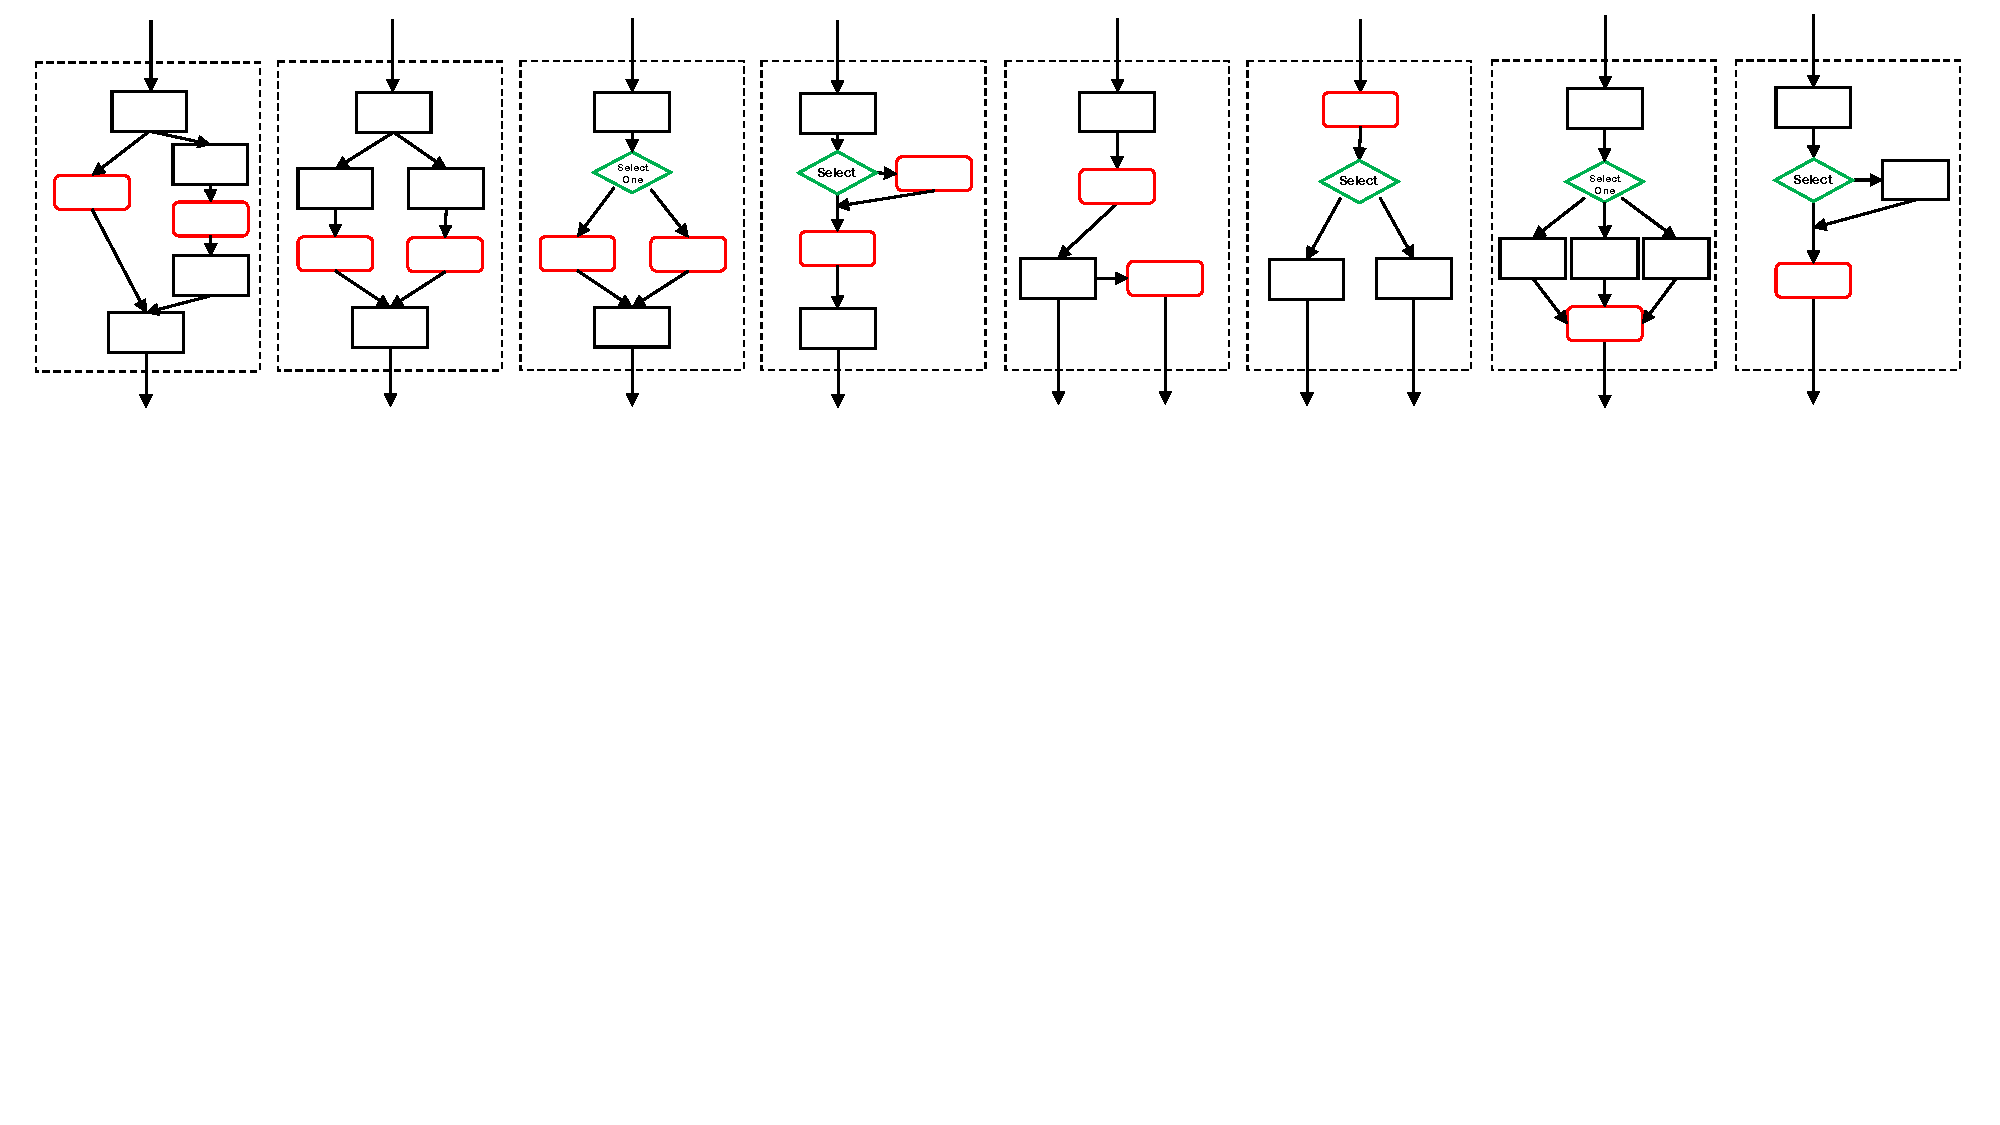
\includegraphics[scale=0.53]{figs/code_composition.pdf}
    \vspace{-10pt}
    \caption{Non-Sequential Code Composition Patterns within Components}
    \label{code_composition}
\end{figure*}

Moreover, we find that composition patterns of code snippets include sequential code composition pattern and various non-sequential composition patterns.
In a typical sequential composition pattern, data is first pre-processed, and then processed by model or rule usage code, and finally post-processed.
The non-sequential code composition patterns are summarized in Fig. \ref{code_composition}. The black box is a data processing code snippet, the red box is a model or rule usage code snippet, and the green diamond means to select one or multiple downstream code snippets.
The first 5 patterns consist of multiple model or rule usages in one component. %, e.g., \textit{ConveRTFeaturizer} component generates sequence and sentence features with two model or rule usages. 
The last 3 patterns consist of a single model or rule usage with multiple possible data processing snippets, decided by configurations or input data.


% \todo{website: add propertion of different code types(data processing code, model usage) in each path.}
% \todo{website: add box figure, for every module, show its Path Num, Pre Num, Pre Line, Post Num, Post Line. For train and predict path, show path num.. (process\_training data). add statistics of different types of code}
% \todo{website: data processing detail type}

\subsection{Implications}
%Our results reflect that the component complexity are from the following aspects.

\textbf{Data processing.} Data processing code is scattered~at~different granularity levels, unlike the well-documented~and~structured code of ML models and rules. 
In detail, data processing code includes data processing components (e.g., \textit{PolicyEnsemble}), general data processing classes and functions in \textit{Shared} module, and specific data processing snippets in components entangled with model or rule usages. 
On the one hand, it could become troublesome to identify and understand the semantics of all data processing code for application developers. A specific example is that data pre-processing code also exists in model definition class of \texttt{TransformerRasaModel}, including \textit{Formant Conversion} and \textit{Data Batch} code. It could be explicitly helpful to automatically extract and analyze the semantics of data processing code  with techniques like program analysis \cite{pycg}. On the other hand, it would be challenging to maintain and test data processing code for system developers, possibly resulting in severe consequences with ML development paradigm shift from model-centric  to data-centric \cite{liangAdvancesChallengesOpportunities2022}. 
In general, building a taxonomy of data processing code would be helpful for the maintaining and testing of data processing code.
% the test oracle of data processing code is hard.


\textbf{Code composition patterns.} These non-sequential composition patterns could introduce additional dynamic complexity for ML-enabled systems, e.g., it is too expensive to capture all possible run-time compositions of code snippets~with~static analysis. Although dynamic testing is widely adopted~to~complement the limitations of static analysis in traditional software \cite{fairley1978tutorial}, most existing testing techniques tailored for ML only target at ML model level \cite{ml_testing}. It would be beneficial to extend them to include data processing code and composition patterns.

% !TeX root = ../main.tex

\section{RQ4: Testing Practice Analysis}
\vspace{-3pt}
\label{sec:test_case}

\subsection{Methodology}

To answer \textbf{RQ4}, test cases were inspected in three steps.

\textbf{Step 1: Label test cases.} We manually labeled the granularity level, oracle type and ML stage of each test case.
There are three different granularity levels of test cases: (1) Method-level: testing single or multiple methods; (2) Component-level: testing the complete process of a component in training~or~inference stage; (3) Integration-level: testing the current component with upstream components. 
There are four test oracle types: (1) Given input-output pairs: the input and expected output data are given; (2) Component-specific constraints: the constraints must be satisfied according to the implementation of a component, i.e., the sum of confidence scores of the intent list generated by classifiers should equal to 1; (3) Differential executions:~outputs of executions under different settings should change or remain the same, i.e., given the same input, the outputs of an original ML model and its loaded version from disk should remain the same; (4) Exception: whether or not the test case throws exceptions for certain inputs and configurations. 
Finally, the ML stages covered by test cases include training, inference and evaluation stages.
To test the training stage of a component, test cases must first train it and check whether any test oracle is violated.
Note that there may exist several oracle types and ML stages but only one granularity level for each test case in Rasa.
Two of the authors labeled test cases independently, and the third author was involved to resolve disagreements. The Cohen's Kappa coefficient of granularity level, test oracle and ML stage is 0.907, 0.908, and 0.854, respectively. 

\textbf{Step 2: Collect code coverage of test cases.} We collected the statement coverage and branch coverage of code via \textit{pytest-cov}, because Rasa uses \textit{pytest} to run test cases. 
% The running time of each test case could be extracted from \textit{pytest} running results directly.


\textbf{Step 3: Collect interaction pattern coverage of test~cases.} We injected logging statements into methods of every component, and then executed test cases to collect the co-executed component sets of each test case. 
All component interaction instances, except \textit{Model Inheritance} instances and some \textit{Usage Constraints} instances that cannot be used together, were tried to be matched with these component sets. 
The matched interaction patterns and instances were considered as covered by test cases.
% For interaction patterns that involve multiple components, we tried to match the longest pattern instance. For example, we matched the set {PolicyEnsemble, RulePolicy}, TEDPolicy with the pattern instance (PolicyEnsemble, (TEDPolicy, RulePolicy)) instead of (PolicyEnsemble, TEDPolicy).

\subsection{Results}

% \todo{add test case running time}
  \begin{table*}[ht]
        \begin{center}
        \caption{Code Coverage and Labeled Statistics of Test Cases}
        \vspace{-5pt}
        \begin{tabular}{cccccccccccccc}
          \hline
          \multirow{2}{*}{\textbf{Module}} &
            \multirow{2}{*}{\textbf{Total}} &
            \multicolumn{3}{c}{\textbf{Test Case Type}} &
            \multicolumn{3}{c}{\textbf{Test Case Stage}} &
            \multicolumn{4}{c}{\textbf{Oracle Type}} &
            \multicolumn{2}{c}{\textbf{Code Coverage}} \\ \cline{3-14} 
           &
             &
            Meth. &
            Comp. &
            Integ. &
            Infer. &
            Train &
            Eval. &
            I-O &
            C-S &
            Diff. &
            Exception &
            Stat. Cov. &
            Bran. Cov. \\ \hline
          \multicolumn{1}{c|}{Tokenizer} &
            \multicolumn{1}{c|}{27} &
            7 &
            20 &
            \multicolumn{1}{c|}{0} &
            25 &
            14 &
            \multicolumn{1}{c|}{0} &
            24 &
            1 &
            0 &
            \multicolumn{1}{c|}{3} &
            97.4\% &
            96.8\% \\
          \multicolumn{1}{c|}{Featurizer} &
            \multicolumn{1}{c|}{62} &
            13 &
            14 &
            \multicolumn{1}{c|}{35} &
            56 &
            40 &
            \multicolumn{1}{c|}{0} &
            46 &
            5 &
            3 &
            \multicolumn{1}{c|}{8} &
            95.7\% &
            94.9\% \\
          \multicolumn{1}{c|}{IntentClassifier} &
            \multicolumn{1}{c|}{36} &
            7 &
            15 &
            \multicolumn{1}{c|}{14} &
            29 &
            30 &
            \multicolumn{1}{c|}{0} &
            18 &
            11 &
            7 &
            \multicolumn{1}{c|}{1} &
            92.5\% &
            89.5\% \\
          \multicolumn{1}{c|}{EntityExtractor} &
            \multicolumn{1}{c|}{41} &
            6 &
            19 &
            \multicolumn{1}{c|}{16} &
            34 &
            31 &
            \multicolumn{1}{c|}{0} &
            18 &
            14 &
            8 &
            \multicolumn{1}{c|}{1} &
            92.3\% &
            90.1\% \\
          \multicolumn{1}{c|}{Selector} &
            \multicolumn{1}{c|}{13} &
            4 &
            6 &
            \multicolumn{1}{c|}{3} &
            9 &
            12 &
            \multicolumn{1}{c|}{0} &
            6 &
            5 &
            1 &
            \multicolumn{1}{c|}{1} &
            68.3\% &
            66.4\% \\
          \multicolumn{1}{c|}{Policy} &
            \multicolumn{1}{c|}{165} &
            77 &
            88 &
            \multicolumn{1}{c|}{0} &
            105 &
            127 &
            \multicolumn{1}{c|}{0} &
            117 &
            51 &
            0 &
            \multicolumn{1}{c|}{20} &
            95.7\% &
            94.5\% \\
          \multicolumn{1}{c|}{Shared} &
            \multicolumn{1}{c|}{138} &
            129 &
            2 &
            \multicolumn{1}{c|}{7} &
            90 &
            84 &
            \multicolumn{1}{c|}{0} &
            89 &
            42 &
            2 &
            \multicolumn{1}{c|}{16} &
            92.3\% &
            91.4\% \\
          \multicolumn{1}{c|}{Total} &
            \multicolumn{1}{c|}{461} &
            240 &
            156 &
            \multicolumn{1}{c|}{65} &
            331 &
            317 &
            \multicolumn{1}{c|}{47} &
            312 &
            123 &
            15 &
            \multicolumn{1}{c|}{49} &
            93.2\% &
            92.0\% \\ \hline
          \end{tabular}
        \label{test_case_statistics}
        \end{center}
        \end{table*}

The code coverage and labeled statistics of test cases are shown in Table \ref{test_case_statistics}. 
(1) The total statement coverage and branch coverage of code reach 93.2\% and 92.0\%, which~is~much higher than 21.5\% and 13.3\% in Apollo \cite{pengFirstLookIntegration2020}. 
(2) The coverage of \textit{Selector} is only 68.3\% and 66.4\%, because \textit{Selector} has two candidate ML models while only one of them was tested. 
% (3) The code coverage of \textit{Tokenizer}, \textit{Featurizer} and \textit{Policy} is higher than that of \textit{IntentClassifier}, \textit{EntityExtractor} and \textit{Shared}, since there are more test cases for them per LoC. 
(3) There are 240 (52.0\%) method-level, 156 (33.8\%) component-level and 65 (14.1\%) integration-level test cases. 
(4) There is no integration-level test cases in \textit{Policy}, because \textit{Policy} was tested with given intents and entities input from developers without the dependency of NLU modules. 
(5) Inference and training stages have similar test case quantities.
(6) Only test cases in \textit{Shared} module cover evaluation stage, because \textit{Shared} module provides the evaluation code for all components.
(7) There are 312 (67.7\%), 123 (26.3\%), 15 (3.3\%), and 49 (10.6\%)~test cases with given input-output pairs, component-specific constraints, differential executions and exception test oracles.

        \begin{table}[!t]
            \caption{Test Coverage of Component Interactions}
            \vspace{-10pt}
            \begin{center}
            \tabcolsep=1.0mm
            \begin{tabular}{llll}
            \toprule
            \textbf{Category}
            & \textbf{Sub-Category}
            & \textbf{Cov. Patterns}
            & \textbf{Cov. Instances} \\
            \midrule
            \multirow{5}*{Inter-module}
            &Data Dependency &9/25 &17/95  \\
            &Confidence Checking &0/2 &0/50  \\
            &Output Selection &0/1 &0/18    \\
            &Output Refinement &1/1 & 1/4   \\
            &Usage Constraints &3/3 &3/3    \\
            \midrule
            \multirow{2}*{Intra-module}
            &Functionality Equivalence &2/2 &3/18  \\
            &Prioriy Order &1/1 &4/7  \\
            &Usage Constraints &2/2 &2/4 \\
            \midrule
            Total
            &  &18/37 &30/199 \\
            \bottomrule
            \end{tabular}		
            \label{component_interaction_coverage}
            \end{center}
        \end{table}

        As Table \ref{component_interaction_coverage} shows, the test coverage of interactions~is~relatively low, i.e., 18 (48.6\%) of 37 patterns and 30 (15.1\%)~of~199 instances are covered. This is because only integration-level tests cover components interactions.
        In particular, \textit{Confidence Checking} and \textit{Output Selection} are not covered.
        % and the coverage of \textit{Data Dependency} is very low. because the tests of them is all at method-level and fcuntion-level.
        
        \subsection{Implications} 
        
        \textbf{Low test coverage of component interactions.} It is difficult to achieve a high test coverage of component interactions,~due to the complexity caused by huge configuration space~and~hidden interactions. The only test cases that cover component~interactions (i.e., integration-level test cases) contribute no more than 15\% test cases.
        Yet, integration-level test cases~can~cover~and kill more mutants than component-level and method-level test cases, as many mutants do not manifest~in~non-integration-level test cases \cite{integration_test}.
        Therefore, it is crucial to generate integration-level test cases for ML-enabled systems.
        
        % which can also be helpful to explore the optimal configurations  
        % the metrics of different pipelines given specific task
        % Although the code coverage of test cases in Rasa is relatively high, the interaction coverage is low.
        % only 14.1\% test cases target at  integration-level.  
        
        \textbf{Limited test oracle types.} 
        It is challenging and time-consuming to write test cases with given input-output pairs and component-specific constraints oracles, due to the complexity brought by lacking of specification for interactions. 
        As~a~result, those test cases without the need of specification of interactions, that is, differential executions and exception test oracles, have been widely utilized to tackle the oracle problem~in~test~case generation techniques for traditional software, such as differential testing \cite{evans2007differential}, fuzzing \cite{liang2018fuzzing} and search-based testing \cite{mcminn2011search}.
        Besides, we find that test cases with these two oracles have a similar capability to kill mutants similar to component-specific constraints oracle (see \textbf{RQ5}). In spite of this, only 13.9\% test cases in Rasa are written with differential executions and exception test oracles, implying that there could be a big room to apply these two test oracle types in test case generation techniques for ML-enabled systems.

% The test oracles of 94.0\% test cases are , which are  for system developers to decide. 
% \todo{test case depend on different configurations, caused by complexity in RQ1 but not covered in RQ4. }
% !TeX root = ../main.tex

\section{RQ5: Mutation Testing Analysis}
\vspace{-3pt}
\subsection{Methodology}

To answer \textbf{RQ5}, we performed an analysis of mutation~testing~\cite{mutation_survey}. 
It applies mutators to generate versions of faulty~code, i.e., mutants. For each mutant, test cases were executed~to~collect the testing results and determine whether~the~mutant~was~killed. %For ML programs, the decision logic is learned from the model definition code, training program and training data, which is why previous ML specific mutation operators also mutate training data, model definition code, hyperparameter, trained model, etc. \cite{DeepMutation,DeepMutation++}. Moreover, the way to decide whether a mutant is killed in ML programs is through performance metrics instead of the running status of test cases like traditional software. 
Since Rasa contains both ML components and rule-based components, we considered mutators for traditional software (i.e., syntactic mutators) as well as ML-specific mutators.
As Table~\ref{mutation_operator} shows, we used 9 syntactic mutators from Jia et al. \cite{JiaMutation} and 11 ML specific mutators from DeepCrime \cite{DeepCrime}. 

We list steps of mutation analysis in the following.

\textbf{Step 1: Generate mutants.}
We generated syntactic mutants using \textit{mutmut} \cite{mutmut}. %which is a Python mutation tool and has been used by \cite{JiaMutation,LibJiaMutation}.
We used two groups of syntactic~mutators, i.e., \textit{Logic} and \textit{Value}, which mutate the logic flow~and~variable value. %(e.g., change ``break" keyword into ``continue") 
 %(e.g., plus the numeric variable value with $1$) of the code, respectively. 
% The mutation tool parses the Python code into Abstract Syntax Tree (AST) and perform possible mutation operators with AST nodes.
Besides, we generated ML specific mutants with DeepCrime \cite{DeepCrime}. 
% which traverses the Python AST and recognize specific Keras API nodes to mutate them (e.g. change the activation function with another Keras API). 
We used 4 of 8 mutation groups in DeepCrime (\textit{Activation}, \textit{Regularization}, \textit{Weights} and \textit{Optimization}). For others, mutators in \textit{Training Data} and \textit{Validation} groups are not the focus of this paper; \textit{Hyperparameters} group is not included, as hyperparameters in Rasa are specified with configuration files by developers; and \textit{Loss Function} group is not applicable,~as the loss functions in Rasa are all implemented from scratch, while the mutators provided by DeepCrime are only to replace the Keras loss function API with another one. Besides, we only generated mutants for 6 labeled code cateogries in \textbf{RQ3}, excluding general utils code. We generated no more than 30 mutants for every Python class to reduce~potential bias. We also only modified one AST node for every mutant.

\textbf{Step 2: Perform mutation testing analysis with test cases.} For every mutant, only test cases that cover the mutated line were collected (from test coverage data in \textbf{RQ4}) and executed to save running time. %We recorded all test case execution~statuses and logs for further analysis. 
If any test case fails on a mutant, the mutant is considered as killed by the test case. Otherwise, the mutant is considered as survived. 
A test case could fail~with three symptoms: (1) an assertion fails; (2) an execution or runtime error manifests; and (3) the test case times out. 
The maximum time for a test case to run is 10 times of its running time in the original clean code version. 
Besides, test cases were executed 3 times for every mutant to avoid flaky tests. We found that all test case statuses remain same for three runs. 
% which shows that test case requires less runs than test data to detect mutants.

\textbf{Step 3: Perform mutation testing analysis with test~data.} For those survived mutants in Step 2, we assessed the impact of them with 3 default configuration files and the restaurant domain data in \textit{Multiwoz} \cite{multiwoz}, which is a widely used multi-domain dataset to evaluate the performance of TDS.
% The Github repo\footnote{https://github.com/razvanra2/ChatBot} was utilized to convert \textit{Multiwoz} into Rasa data format and  are adopted to train the Rasa pipeline.
Given a configuration file, only components specified in it are included in the Rasa pipeline, thus mutated nodes of some survived mutants from Step 2 will not be executed~as~they~are~not~\textit{impacted} by the configuration.
Due to the stochastic nature of machine learning programs, we trained both the mutated program and original program for 5 times with 80/20 data split into train/test data randomly, and decided whether the performance metrics of two versions are statistically significant with non-negligible and non-small effect size.
We followed the same formula to decide whether a mutant is killed with the test data as \cite{mutation_evaluation, DeepCrime}, with the threshold of significance value is 0.05 and of effect size is 0.5.
% and we trained the Rasa pipeline with 100\%/75\%/25\% training data separately to investigate the performance degeadation of mutants with different amount of training data.
We adopted F1 scores of \textit{IntentClassifier}, \textit{EntityExtractor} and \textit{Policy} as performance metrics, i.e., if the F1 score in any of the three modules is statistically different between two code versions, the mutant is marked as killed by test data.
\subsection{Results}


% \todo{website: add detail analysis of test dataset(error analysis) }

\begin{table}[]
  \tabcolsep=1.0mm
  \begin{center}
  \caption{Mutation Testing Results}
  \vspace{-5pt}
  \begin{tabular}{ccccccc}
  \hline
  \multirow{2}{*}{\textbf{Mutation Group}} & \multirow{2}{*}{\textbf{Operator}} & \multirow{2}{*}{\textbf{Total}} & \multicolumn{2}{c}{\textbf{Test Case}} & \multicolumn{2}{c}{\textbf{Test Data}} \\ \cline{4-7} 
                                                       &                            &                       & Killed & Survived              & Impacted & Killed  \\ \hline
  \multicolumn{1}{c|}{\multirow{6}{*}{Logic}}          & \multicolumn{1}{c|}{ArOR}  & \multicolumn{1}{c|}{109} &86        & \multicolumn{1}{c|}{23} &10          & 1 \\
  % \multicolumn{1}{c|}{}                                & \multicolumn{1}{c|}{BitOR} & \multicolumn{1}{c|}{} &        & \multicolumn{1}{c|}{} &          &         \\
  \multicolumn{1}{c|}{}                                & \multicolumn{1}{c|}{ComOR} & \multicolumn{1}{c|}{109} &88        & \multicolumn{1}{c|}{21} &6          &0         \\
  \multicolumn{1}{c|}{}                                & \multicolumn{1}{c|}{LogOR} & \multicolumn{1}{c|}{145} &112        & \multicolumn{1}{c|}{33} &14          &0         \\
  \multicolumn{1}{c|}{}                                & \multicolumn{1}{c|}{AsOR}  & \multicolumn{1}{c|}{20} &19        & \multicolumn{1}{c|}{1} &0          &0         \\
  \multicolumn{1}{c|}{}                                & \multicolumn{1}{c|}{MemOR} & \multicolumn{1}{c|}{32} &30        & \multicolumn{1}{c|}{2} &0          &0         \\
  \multicolumn{1}{c|}{}                                & \multicolumn{1}{c|}{KVR}   & \multicolumn{1}{c|}{12} &7        & \multicolumn{1}{c|}{5} &1          &0         \\ \hline
  \multicolumn{1}{c|}{\multirow{3}{*}{Value}}          & \multicolumn{1}{c|}{BVR}   & \multicolumn{1}{c|}{64} &32        & \multicolumn{1}{c|}{32} &9          &0         \\
  \multicolumn{1}{c|}{}                                & \multicolumn{1}{c|}{NVR}   & \multicolumn{1}{c|}{224} &180        & \multicolumn{1}{c|}{64} &18          &2         \\
  \multicolumn{1}{c|}{}                                & \multicolumn{1}{c|}{AsVR}  & \multicolumn{1}{c|}{582} &525        & \multicolumn{1}{c|}{67} &10          &0         \\ \hline
  \multicolumn{1}{c|}{\multirow{3}{*}{Activation}}     & \multicolumn{1}{c|}{ACH}   & \multicolumn{1}{c|}{22} &3        & \multicolumn{1}{c|}{19} &18          &6         \\
  \multicolumn{1}{c|}{}                                & \multicolumn{1}{c|}{ARM}   & \multicolumn{1}{c|}{2} &0        & \multicolumn{1}{c|}{2} &1          &0         \\
  \multicolumn{1}{c|}{}                                & \multicolumn{1}{c|}{AAL}   & \multicolumn{1}{c|}{22} &11        & \multicolumn{1}{c|}{11} &11          &2         \\ \hline
  \multicolumn{1}{c|}{\multirow{3}{*}{Regularization}} & \multicolumn{1}{c|}{RAW}   & \multicolumn{1}{c|}{6} &0        & \multicolumn{1}{c|}{6} &3          &3         \\
  \multicolumn{1}{c|}{}                                & \multicolumn{1}{c|}{RCW}   & \multicolumn{1}{c|}{10} &0        & \multicolumn{1}{c|}{10} &10          &0         \\
  \multicolumn{1}{c|}{}                                & \multicolumn{1}{c|}{RRW}   & \multicolumn{1}{c|}{5} &0        & \multicolumn{1}{c|}{5} &5          &0         \\ \hline
  \multicolumn{1}{c|}{\multirow{3}{*}{Weights}}        & \multicolumn{1}{c|}{WCI}   & \multicolumn{1}{c|}{24} &10        & \multicolumn{1}{c|}{14} &13          &1         \\
  \multicolumn{1}{c|}{}                                & \multicolumn{1}{c|}{WAB}   & \multicolumn{1}{c|}{4} &0        & \multicolumn{1}{c|}{4} &3          &1         \\
  \multicolumn{1}{c|}{}                                & \multicolumn{1}{c|}{WRB}   & \multicolumn{1}{c|}{3} &1        & \multicolumn{1}{c|}{2} &2          &0         \\ \hline
  \multicolumn{1}{c|}{\multirow{2}{*}{Optimization}}   & \multicolumn{1}{c|}{OCH}   & \multicolumn{1}{c|}{24} &2        & \multicolumn{1}{c|}{22} &9          &6         \\
  \multicolumn{1}{c|}{}                                & \multicolumn{1}{c|}{OCG}   & \multicolumn{1}{c|}{8} &0        & \multicolumn{1}{c|}{8} &3          &0         \\ \hline
  \multicolumn{1}{c|}{\multirow{1}{*}{Total}}   & \multicolumn{1}{c|}{}   & \multicolumn{1}{c|}{1447} &1106        & \multicolumn{1}{c|}{341} &146          &22         \\ \hline
  \end{tabular}
  \label{mutation_operator}
  \end{center}
  \end{table}
  
  % \todo{add merged results of 100\%, 75\% and 25\% killed.}

  The mutation testing results by each mutator are shown~in Table \ref{mutation_operator}. There are 1447 mutants generated, 1106 (76.4\%)~mutants killed by test cases, 341 (23.6\%) mutants survived, 146 (10.1\%) mutants impacted, and 22 (1.5\%) mutants killed by test data. 
  Only 146 mutants from 341 survived mutants impact the default 3 Rasa pipelines, which shows that the huge configuration space is challenging to be tested  adequately.
  81.3\% syntactic mutants and 20.0\% ML specific mutants are killed by test cases, while 4.4\% syntactic mutants and 24.4\% ML specific mutants from impacted mutants are killed by test data.
  It shows that test case is much more effective to detect syntactic mutants and slightly less effective to detect ML specific mutants than test data. 
  % because \textit{ML specific mutants} are more like \textit{mis-configuration problems} than \textit{bugs} in traditional softwares.
  The killed syntactic mutants and ML-specific mutants by test data cause the F1 score degradation of \textit{IntentClassifier}, \textit{EntityExtractor} and \textit{Policy} by 20.8\%, 0.8\%, 3.6\% and 11.1\%, 13.4\%, 5.7\% on average.

  %1079/(248+1079) = 81.3%, 26/130 =20%, 3/68= ,  19/78=
  
  % However, more mutants are killed with 75\% training data than with 25\% training data, because the performance metrics are poor even in clean Rasa code version with 25\% training data.
  % \todo{should see the assert error killed by test data(more fair to compare the ability between test case and test data). }
  
  % \todo{any mutants killed by test cases(assertion error), the impact on test data?}

  \begin{table}[!t]
  \begin{center}
  \caption{Mutant Location Results}
  \vspace{-5pt}
  \scalebox{1}{
    \begin{tabular}{cccccc}
      \hline
      \multirow{2}{*}{\textbf{Location}} & \multirow{2}{*}{\textbf{Total}} & \multicolumn{2}{c}{\textbf{Test Case Result}} & \multicolumn{2}{c}{\textbf{Test Data Result}} \\ \cline{3-6} 
                                       &                          & Killed & Survived                 & Impacted & Killed \\ \hline
      \multicolumn{1}{c|}{Data Prep.}  & \multicolumn{1}{c|}{385} & 326    & \multicolumn{1}{c|}{59}  & 23       & 0      \\
      \multicolumn{1}{c|}{Data Post.}  & \multicolumn{1}{c|}{271} & 222    & \multicolumn{1}{c|}{49}  & 5        & 0      \\
      \multicolumn{1}{c|}{Model Usage} & \multicolumn{1}{c|}{307} & 243    & \multicolumn{1}{c|}{64}  & 4        & 0      \\
      \multicolumn{1}{c|}{Model Def.}  & \multicolumn{1}{c|}{364} & 224    & \multicolumn{1}{c|}{140} & 99       & 22     \\
      \multicolumn{1}{c|}{Rule Usage}  & \multicolumn{1}{c|}{4}   & 4      & \multicolumn{1}{c|}{0}   & 0        & 0      \\
      \multicolumn{1}{c|}{Rule Def.}   & \multicolumn{1}{c|}{115} & 101    & \multicolumn{1}{c|}{14}  & 4        & 0      \\ \hline
      \end{tabular}}
    \label{mutation_location}
    \end{center}
    \end{table}

  The mutation testing results w.r.t. the location of mutants are shown in Table \ref{mutation_location}. 224 (61.5\%) of 364 mutants in model definition code, and 896 (82.8\%) of 1082 mutants in other code categories are killed by test cases. 
  In particular, few mutants in code categories except model definition are impacted and killed by test data, which implies that test data is only effective to kill mutants in model definition code.

   
    \begin{table}[!t]
        \begin{center}
          \tabcolsep=1.0mm
            \caption{Test Case Mutation Results}
            \vspace{-5pt}
        \scalebox{0.95}{
        \begin{tabular}{c|c|cccc}
        \hline
        \textbf{Category} & \textbf{Type} &\textbf{Test Num.} &\textbf{Strong Test Num.}     & \textbf{Covered}        &\textbf{Killed}  \\ \hline
        \multirow{3}{*}{Granularity}   & Method &240 &59 &947     & 635      \\
                                          & Component &156 &31 &1121       &709     \\
                                          & Integration &65 &29 &903    &613      \\ \hline
        \multirow{4}{*}{Stage}  & Infer. &331 &86 &1358           &995      \\
                                          & Training &317 &75 &1184        &847      \\
                                          & Evaluation &47 &11 &772 &476       \\ \hline
        \multirow{4}{*}{Oracle Type}  & I-O &312 &98 &1298    &956      \\
                                          & C-S  &123 &19 &1103  &707      \\
                                          & Diff &15 &3  &625   &338    \\
                 & Exception &49  &6 &686 &352   \\ \hline
        \end{tabular}}
        \label{test_mutation}
    \end{center}
        \end{table}
    
    We investigated the capability to detect mutants~w.r.t.~different categories of test cases, by calculating the ratio of \textit{strong test case number} to \textit{all test case number}, and the ratio of \textit{killed mutants} to \textit{covered mutants} of them.  
    We define \textit{strong test case} as the test case that kills equal or more than 75\% of its covered mutants. 
    As Table \ref{test_mutation} shows, test cases in integration level have the highest ratio of strong test case (44.6\%) and highest ratio of killed mutants (67.9\%) among three granularity levels.
    Test cases with given input-output test oracle have the highest ratio of strong test case (31.4\%)  and highest ratio of killed mutants (73.7\%) among four oracle types, while test cases with other three oracle types have similar ratios.  


%  \todo{}
%        \begin{table}[!t]
%          \tabcolsep=1.0mm
%            \begin{center}
%                \caption{Test Module with Mutant Module Analysis}
%                \vspace{-5pt}
%            \scalebox{0.95}{
%            \begin{tabular}{c|cccccc}
%            \hline
%            \textbf{Test \textbackslash{} Mutant Module} & To. & Fe. & In. & En. & Se. & Po.  \\ \hline
%            Tokenizer        &41/46 &0  &0  &0  &0  &0    \\
%            Featurizer       &28/31                       &164/180  &0  &0  &0  &0     \\
%            IntentClassifier &24/32                       &60/96  &101/147  &4/19  &0  &0      \\
%            EntityExtractor  &24/30                       &10/18  &44/59  &110/141  &0  &0      \\
%            Selector         &21/26                       &44/74  &29/42  &0  &15/19  &0      \\
%            Policy           &0                       &0  &0  &0  &0  &252/307    \\
%            Diff & 3/6 & 20/20 & 8/12 & 1/3 & 0 & 0 
%            \\
%                                                      \hline
%            \end{tabular}}
%            \label{test_module}
%        \end{center}
%            \end{table}
  
%  To evaluate the capability of integration-level test cases in Rasa, we computed the relations of module of test case and its killed/covered mutants, and the results are shown in Table \ref{test_module}.
%  The \textit{Diff} row presents the number of mutants in each module that can not be killed/covered by component-level and method-level tests, and can only be killed/covered by integration-level tests.
%  There are 32/41 mutants can only be killed/covered by integration tests in total.
%  We also found that no mutants that killed/covered by other tests can not be killed/covered by integration-level tests. 
%  % For example, integration-level test cases that aim to test \textit{IntentClassifier} can also detect mutants located in \textit{Featurizer}, because it may call \textit{Featurizer} to process input data.     
%  It is harder for downstream modules (e.g. \textit{Policy}) to be tested than upstream modules, because there are no integration-level test cases for them. 

\subsection{Implications}

\textbf{Non-ML specific bugs and test cases in ML-enabled~systems.} 
Complexity arising from data processing code increases the likelihood of introducing non-ML specific bugs.
% As Table \ref{code_type_stat} shows, the ML model usage and definition code only contributes 33.5\% LoC of all ML-related code, thus lots of non-ML specific bugs are prone to be introduced in data processing, rule usage and rule definition code. 
Compared to test data, test case is more effective to detect syntactic mutants, i.e., non-ML specific bugs.
Moreover, it is notorious~for~developers to analyze, localize and fix bugs in ML programs based on test data alone, leading to the development of interpretation \cite{interpretability}, debugging \cite{abid2022meaningfully} and repairing \cite{sun2022causality} techniques for ML models. 
It is easier for developers to localize and fix bugs with failed test cases by analyzing violated test oracles.
Thus, we argue that non-ML specific bugs and test cases in  ML-enbaled systems should received greater attention.
Although there~is~a~rich~set of test cases in Rasa that achieve high code coverage, the mutant kill ratio remains to be improved (76.4\%), particularly for ML-specific mutants (29.8\%).
The applicability and limitations of existing test case generation, selection and quality assurance techniques in ML-enabled systems are worthwhile to be explored \cite{kazmi2017effective, di2013coverage}. 

% \textbf{Challenges of test case to kill mutants.}
% Besides, interation-level test case is helpful
% most effective to cover and kill mutants, but less in test suite.
% More efforts should be paied to generate more integration-level test cases.
% 

\textbf{Challenges of test data to kill mutants.}
Existing researches on mutation testing for ML programs only evaluated mutants with test data to determine whether mutants can be killed~\cite{DeepCrime,DeepMutation++,DeepMutation,mutation_evaluation,JiaMutation}.
However, the capability of test data to kill mutants in large-scale ML-enabled systems is limited for two reasons.
First, due to complexity from configurations, only a subset of mutants will impact the components of actual configured systems.
Second, the quantity and distribution of training data and test data affect the results a lot.
For example, we attempted to train the clean code version and mutated version with 75\% of original training data, and the number of killed mutants changed from 22 to 83, which means some bugs may only manifest under specific training data settings. 
Therefore, system developers should evaluate and test ML-enabled systems under a wider range of configurations and data settings that may be employed by application developers to detect potential bugs.%, which is especially important for safety-critical systems.

% Question: \textbf{Integration-level test can not be replace by component-level and method-level tests.} add here?


% bug in xx place is harder to be killed, in xx place cause most performance degration.
% test case targets at training stage cost too much time.
% !TeX root = ../main.tex
\section{threats}
\vspace{-3pt}

First, our study conducts a case study on Rasa, a widely~used task-oriented industrial dialogue system. It is not clear whether our results can be generalized to other ML-enabled systems. However, we believe it is a good start to take a system view~for ML-enabled systems. Second, our study involves~a~lot~of~manual analyses of Rasa source code and documentations, which may incur biases. To reduce them, two of the authors conduct manual analysis separately, and a third author is involved to resolve disagreements. Third,~the~mutators~that we adopt~may not simulate real-world bugs. To mitigate it,  we decide~to~use mutators from DeepCrime \cite{DeepCrime}, whose mutators are actually summarized from real word ML bugs. 
% Further, the configuration files we 
% !TeX root = ../main.tex

\section{Related Work}
\vspace{-3pt}

\textbf{Study of ML-Enabled Systems}. While much of the attention has been on ML models, less attention has been paid on system-level analysis~\cite{Christian2022}. Peng et al.~\cite{pengFirstLookIntegration2020} investigated~the~integration of ML models in Apollo by analyzing how ML models~interact with the system and how is the current testing effort. Besides, Nahar et al.~\cite{Nahar2022} explored collaboration challenges between data scientists and software engineers through interviews.~Amershi et al.~\cite{Amershi2019} and Bernardi et al.~\cite{Bernardi2019} reported~challenges and~practices of MLOps (from model requirement~to~model~monitoring) at Microsoft and Booking.com. Although they~still~take~a~model-centric view,~they~emphasize~that~models can~be~complexly~entangled to cause non-monotonic~errors~\cite{Amershi2019} and model quality~improvement does not necessarily indicate system value~gain~\cite{Bernardi2019}. Further, Yokoyama~\cite{Yokoyama2019} developed an architectural pattern to separate ML and non-ML components, while Serban~and~Visser \cite{Serban2022} surveyed architectural challenges for ML-enabled systems. Sculley et al.~\cite{hidden_technical_debt} identified ML-specific technical debt~in~ML-enabled systems, while Tang et al.~\cite{tang2021empirical} further derived new~ones from real-world code refactorings. In addition, some attempts were made on the problem of ML component entanglement~\cite{Amershi2019}, e.g., performing metamorphic testing on a system with two~ML components~\cite{Zhang2016}, troubleshooting failures in a system with~three ML components by human intellect~\cite{nushi2017human}, and decomposing~errors in a system with two or three ML components~\cite{fix_that_fails}. These studies explore the interaction among models but only~on~simple systems. Moreover, Abdessalem et al.~\cite{Abdessalem2018, Abdessalem2020} studied the feature interaction failures in self-driving systems, and proposed testing and repairing approaches to automatically detect and fix them. Apel et al.~\cite{feature_interaction} also discussed feature interactions in ML-enabled systems, and suggested strategies to cope with them.

The main difference from the previous work is that we~take~a large-scale complex ML-enabled system, explore its complexity at three levels, and analyze the impact of its complexity~on~testing. The closest work is Peng et al.'s~\cite{pengFirstLookIntegration2020}, but we report~a~deeper complexity analysis and also conduct a testing impact analysis.

\textbf{Mutation Testing for DL Models}. Jia et al.~\cite{JiaMutation}~used~syntactic mutators for traditional programs to DL models.~DeepMutation \cite{DeepMutation} and DeepMutation++~\cite{DeepMutation++} defined DL-specific mutators. DeepCrime~\cite{DeepCrime} derived DL-specific  mutators based~on real~DL bugs. 
Jahangirova and Tonella~\cite{mutation_evaluation} evaluated syntactic and DL-specific mutators. These studies are focused on model-level mutation, while we target at system-level mutation.

\textbf{Testing for Dialogue Systems}. Bozic and Wotawa~\cite{Bozic2018}~proposed a security testing approach for chatbots to prevent cross-site scripting and SQL injection. Bozic et al.~\cite{Bozic2019a}~tested a hotel booking chatbot via planning. Bozic and Wotawa~\cite{Bozic2019b}~introduced a metamorphic testing approach for chatbots. Similarly, Liu et al.~\cite{liu2021dialtest} used semantic metamorphic relations to test the NLU module in dialogue systems. Despite the effort,~less~attention has been paid on system-level testing of dialogue systems.


% !TeX root = ../main.tex

\section{conclusion}
\vspace{-3pt}

%\section{Data Availability}

We present a comprehensive study on Rasa to characterize its complexity at three levels and the impact of its complexity on testing from two perspectives.
Furthermore, we highlight practical implications to improve software engieering for ML-enabled systems.
All study data and source code used in this paper are available at \url{https://rasasystemcomplexity.github.io/}.


%\clearpage

{\footnotesize
\bibliographystyle{IEEEtranS}
\bibliography{IEEEabrv, src/reference}
}

\end{document}
\endinput